%!TEX root = ../report.tex

\newcommand\scalemath[2]{\scalebox{#1}{\mbox{\ensuremath{\displaystyle #2}}}}


\begin{document}
    \chapter{Evaluation and Experimental Result}
	\label{chap:evaluationandresult}
    Evaluation and experimental result chapter contains the metrics used to evaluate the conducted experiment and the discussion on the research questions. Results of research question is answered in the subsequent sections with listing of the result in a table. Three research questions answered in the section are the results of state of the art temporal fusion techniques, How are the results in comparison to each other and finally cross transfer the temporal fusion techniques from depth estimation to the semantic segmentation. The model is trained and evaluated on three datasets Scannet \cite{79_dai2017scannet}, Virtual kitti \cite{80_cabon2020vkitti2} and VIODE \cite{81_minodaRAL2021} datasets. 
    
    \section{Evaluation Metric}
    
    The proposed model needs to be validated to understand the impact of the newly trained model. To validate the model different evaluation metrics are proposed. The description of the proposed model is listed below.
    \subsection{Pixel Accuracy}
    
    Pixel accuracy is commonly defined as percent of pixels in a image correctly classified into a particular class. Accuracy is defined as below
    
    $
    {\bf Accuracy } = \scalemath{2}{\frac{TP+TN}{TP+TN+FP+FN}}
    $
    
    where
     
    $TP$ = True Positive 
    
    $TN$ = True Negative
    
    $FP$ = False Positive
    
    $FN$ = False Negative
    
    
    Per class mean pixel accuracy (mPA)
    
    Per class mean pixel accuracy is the average of pixel accuracies of all the classes.
    
    Pixel accuracy (PA) and Mean pixel accuracy (mPA) can also be defined as below \cite{84_ulku2022survey}
    
    $
    {\bf PA } = \scalemath{2}{\frac{\sum_{j=1}^{k} n_{jj}}{\sum_{j=1}^{k} t_j} }
    $
    
    $
    {\bf mPA } = \scalemath{2}{\frac{1}{k} \frac{\sum_{j=1}^{k} n_{jj}}{\sum_{j=1}^{k} t_j}}
    $
    
    where $n_{jj}$ is the total number of pixels both classified and labeled as class $j$. 
    
    \subsection{IoU}
    
    Intersection over Union (IoU) also known as the Jaccard index is a method to quantify the overlapping between the target mask and the predicted output. In other words, it is number of pixels common between the target and prediction masks by the total number of pixels exist between both the masks \cite{83_iou}. pictorial representation of the same is presented in Fig \ref{fig:IoU}
    
    \begin{figure}[h]
    	\centering
    	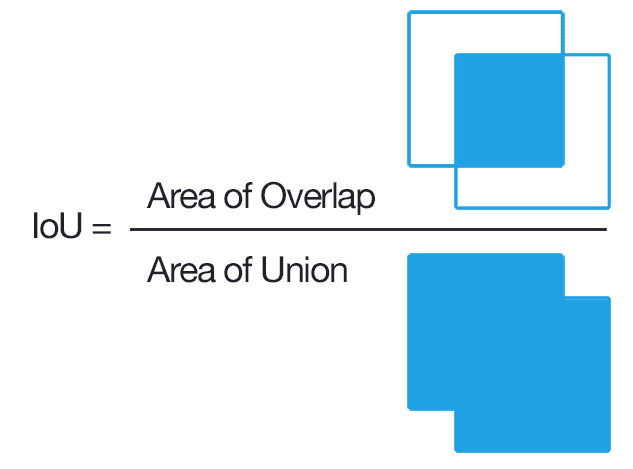
\includegraphics[width=12cm]{images/IoU.png}
    	\caption{IoU. Courtesy of \cite{82_iou}}
    	\label{fig:IoU}
    \end{figure}  
	
	IoU is calculated for each class separately and then averaged over all the classes to provide mean IoU.  
	
	$
	{\bf IoU} = \scalemath{2}{\frac{\sum_{j=1}^{k} n_{jj}}{\sum_{j=1}^{k} (n_{ij}+n_{ji}+n_{jj})}, i \neq j }
	$

	where $ n_{ij}$ is the pixels which are labeled as class i but classified as class j and $n_{ji}$ is the total number of pixels labeled as class j, but classified as class i. \cite{84_ulku2022survey}
	
	$
	{\bf mIoU} = \scalemath{2}{\frac{1}{k} \sum_{j=1}^k \frac{n_{ij}}{n_{ij}+n_{ji}+n_{jj}},  i \neq j }
	$
	
	Frequency weighted IoU (FwIoU). It is a metric derived from the mIoU which weighs each class importance depending on appearance frequency using $t_j$ \cite{84_ulku2022survey}
	
	$
	{\bf FwIoU} = \scalemath{2} {\frac{1}{\sum_{j=1}^k t_j} \sum_{j=1}^{k} t_j \frac{n_{jj}}{n_{ij}+n_{ji}+n_{jj}}, i \neq j }
	$
    
    \section{Hypothesis}
    
    Semantic segmentation is a vital task in the computer vision domain that assigns labels to every pixel in an image. Semantic segmentation is applied in 2D images, Video data, and 3D or Volumetric data. The video sequence data contains multiple image frames stacked together. Given the high frame rate of the video, the consecutive frames are related to each other due to the overlapping regions in the successive frames. In most semantic segmentation tasks, the segmentation is performed on each frame or the keyframes. Past information can be fused into current step computation by taking the learned features from previous frames \cite{78_hu2020temporally}.
    
    The work hypothesizes that the performance improves by fusing the past information onto the current frame segmentation computation by the following approaches.
    
    (i) Subjecting the latent space encoding of the Unet model to the Gaussian process by taking the pose of the current frame and the previous frame, the performance improves in comparison to segmentation without temporal fusion since the overlapping information present in the past is used for computation of the current frame segmentation.
    
    (ii) Placing the ConvLSTM cell at the latent space encoding of the Unet model to transfer the geometry information from the past to the current step helps improve semantic segmentation performance. 
    
    The approach is cross-transferred from the depth estimation task \cite{52_hou2019multi} \cite{03_duzceker2021deepvideomvs}. 
    
    \section{RQ1: What are the works on state-of-the-art temporal fusion in semantic segmentation?}
	
	Segmentation is the process of assigning pixel labels for a given image. Segmentation can be observed in different context such as Video instance segmentation (VIS), Semantic segmentation of the key frames of a video sequence, Video panoptic segmentation, MRI image segmentation, autonomous driving scene understanding. Youtube - Video Instance Segmentation (VOS), Scannet are the common datasets in the semantic segmentation domain. 
	
	{ \bf Youtube VIS data}
	Youtube - Video Instance Segmentation (VIS) is a dataset that extends the image instance segmentation from the image to the video domain. The dataset aims to solve the problem of simultaneous detection, segmentation and tracking problem. Scannet is an RGB-D video dataset containing 2.5 millions views with more than 1500 scans. 
%	\ref{59_starck2005image}
	A paper by Xiang Li et.al [87] explains the temporal fusion for online video instance segmentation. The author introduced the concept of an online video framework with novel aware temporal fusion method. A cropping free temporal fusion approach to model the temporal consistency between video frames. A bottom-up online transformer based network is used to solve the VIS problem. A transformer layer is introduced in the convolutional neural network (CNN) to include the instance information. A attention layer between the frames used to extract the instance code for the current frame. A skip connection is used to use low level contextual information and use dynamic convolution to generate the segmentation map. CNN feature map and the latent code combined together helps to jointly represent instance aware features. A instance code is a LxD vector to VIS task, where L is the maximum detected instances number in a frame D is the feature instance for each instance. Inter and intra frame attention module for fusing the temporal information. The network architecture is presented in Fig \ref{fig:vis}. Three types of attention code-to-code(c2c), code-to-pixel(c2p), and pixel-to-code(p2c) used to construct the	relation between the instance code and feature map. Inter frame used to build the temporal correlation and combine contextual features across frames. Inter frame c2c, c2p and p2c are used to construct the temporal information.
	
    \begin{figure}
		\centering
		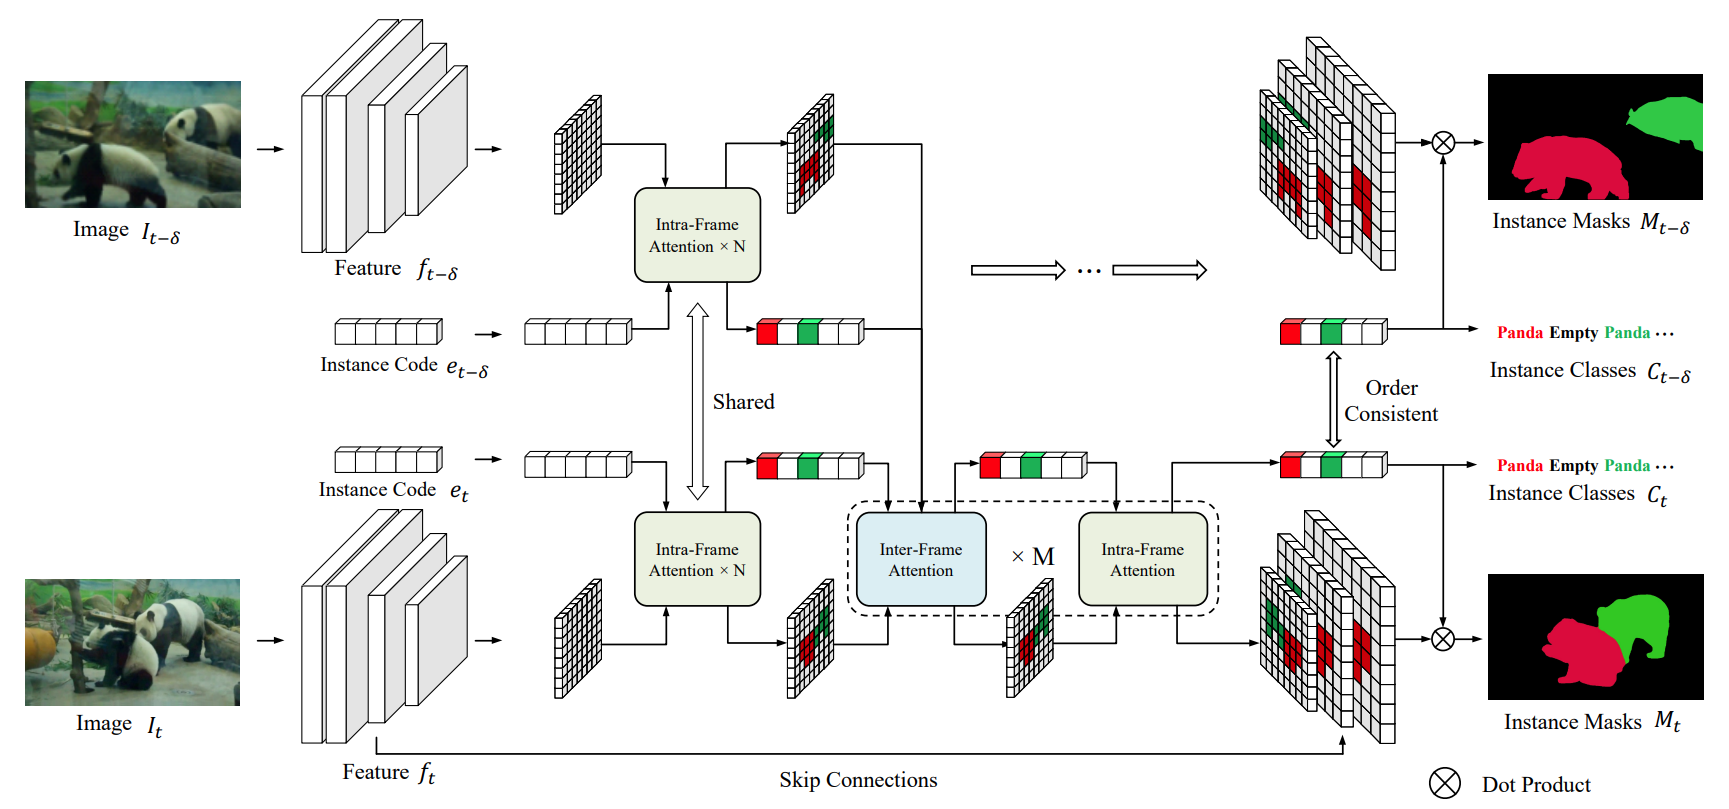
\includegraphics[width=13cm]{images/VIS.png}
		\caption{VIS proposed framework. Courtesy of [87]}
		\label{fig:vis}
	\end{figure}
%	\ref{87_heo2022vita}
	Miran Heo et al [88] worked on the video instance segmentation via Object Token Association (VITA). The work effectively understand the video by the object centric tokens. The VITA model requires a frame-level detector. The frame level detector localizes instances using masks without the need of bounding boxes. Two features is generated for the frame-level predictions specifically: a) dynamic 1x1 convolution weight from the frame queries f b) per-pixel embeddings from the pixel decoder. Dot product between the two embeddings are taken in the frame-level predictions. The end-to-end video instance segmentation method VITA is divided into three stages. Firstly, VITA works with the frame-level detector in a manner that is frame independent. No computation between the frames are involved. The frame queries that holds the object centric information are collected throughout the video sequence and object encoder is used to build the video level information between the frames. And thirdly the decoder combines the information from the frame and video queries which is finally used to find the object mask in the video frames. 
	
	\begin{figure}
		\centering
		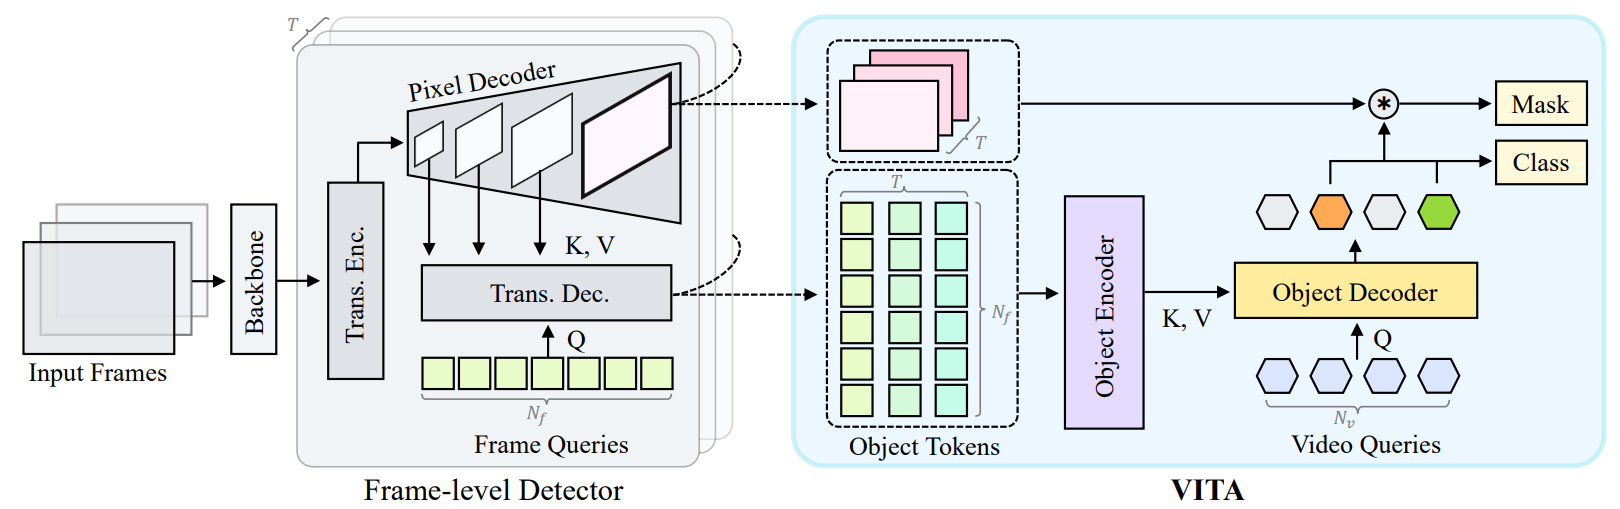
\includegraphics[width=13cm]{images/VITA.png}
		\caption{The frame level detector take frame queries and mask features and generate the embeddings and pass onto the VITA model for mask prediction. The object-aware knowledge in the spatial scenes is captured by construction of the temporal interactions between the frame queries. Finally mask trajectories are obtained form the VITA model. Courtesy of [88]}
		\label{fig:vita}
	\end{figure}
%	\ref{88_huang2022minvis}
	A minimal video instance segmentation (MinVIS) by De-An Huang et al [89] does not require video based training and can be applied directly to image containing sparse image instance segmentations annotations. MinVIS is a two stage approach: 1) Independent image instance segmentation on each frame 2) Instance association between the frames. Image Instance Segmentation has three unique main components a)Encoder to extract features from the image b) Transformer decoder, used to process the output of image encoder to update the query embeddings c) Prediction head takes the query embeddings to predict the output. Association between the instance segmented frames is calculated by bipartite matching of the respective query embeddings.   
	
	\begin{figure}
		\centering
		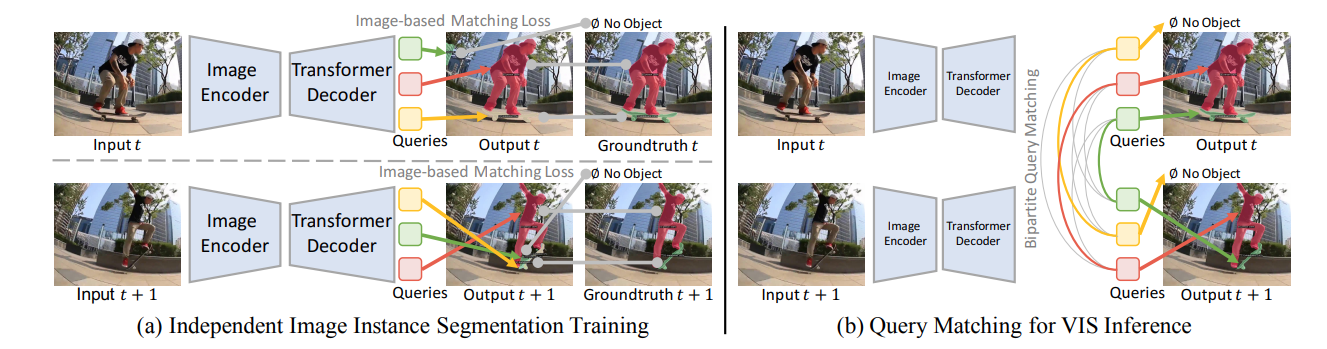
\includegraphics[width=13cm]{images/minVIS.png}
		\caption{(a) MinVIS trained on query based segmentation individually for every frame. (b) Inference of the video instance segmentation from the segmented image using bipartite matching of th query embeddings. Courtesy of [89] }
		\label{fig:minVIS}
	\end{figure}
%	\ref{89_cheng2021mask2former}
	Mask classification in image segmentation problem is solved by the state of the art segmentation models. B.Cheng et al [90] proposed a method to process directly the video rather than the image. This is achieved by feeding the Mask2Former with 3D spatio-temporal features and predict the 3D volume to track each object instances across time. For data with single frame the Mask2Former works as a general image segmentation model. For data with more than 1 frame the model segments and tracks instances across frames. 

	\begin{figure}
		\centering
		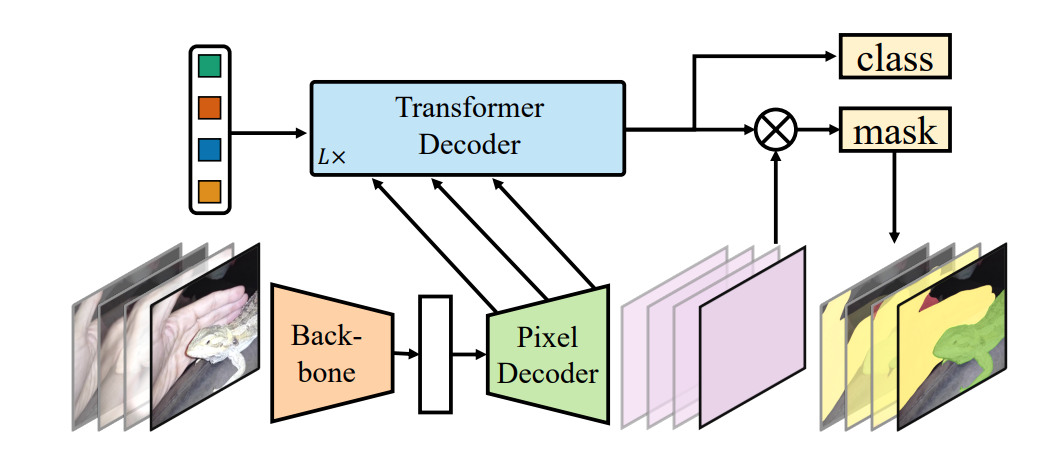
\includegraphics[width=13cm]{images/mask2former.png}
		\caption{ A mask2former with video instance segmentation. Courtesy of  [90]}
		\label{fig:mask2former}
	\end{figure}	
	
    \section{RQ2: How are the results from RQ1 compared with each other to perform temporal fusion?}
    
   	All of the above mentioned approaches are trained and tested on the Youtube VIS datasets. The performance of the models are tabulated in table \ref{tab:sota_ytube_vis}.
   
	\begin{table}[h]
   		\begin{center}
   			\begin{tabular}{ | l | l| l| l| l| p{2cm} |}
   				\hline
   				
   				\cellcolor{purple!30}Method & \cellcolor{purple!30}AP & \cellcolor{purple!30}AP50 & \cellcolor{purple!30}AP75 & \cellcolor{purple!30}AR1 & \cellcolor{purple!30}AR10 \\ \hline
%   				\ref{86_li2022hybrid}
   				HIATF for VIS 2019 [87] & 41.3 & 61.5 & 43.5 & 42.7 & 47.8 \\ \hline
%   				\ref{87_heo2022vita}
   				VITA ResNet-50 2019 [88]  & 49.8 & 72.6 & 54.5 & 49.4 & 61.0  \\ \hline
%   				\ref{87_heo2022vita}
   				VITA ResNet-101 2019 [88]  & 51.9 & 75.4 & 57.0 & 49.6 & 59.1 \\ \hline
%   				\ref{87_heo2022vita}
   				VITA Swin-L 2019 [88]  & 63.0 & 86.9 & 67.9 & 56.3 & 68.1 \\ \hline
%   				\ref{87_heo2022vita}
   				VITA 2021 [88]  & 45.7 & 67.4 & 49.5 & 40.9 & 53.6 \\ \hline
%   				\ref{88_huang2022minvis}
   				Min VIS 2019 [89] & 61.6 & 83.3 & 68.6 & 54.8 & 66.6 \\ \hline
%   				\ref{88_huang2022minvis}
   				Min VIS 2021 [89] & 55.3 & 76.6 & 62.0 & 45.9 & 60.8 \\ \hline
%   				\ref{89_cheng2021mask2former}
   				Mask2former 2019 [90]  & 60.4 & 84.4 & 67.0 & - & - \\ \hline
%   				\ref{89_cheng2021mask2former}   
   				Mask2former 2021 [90]  & 52.6 & 76.4 & 57.2 & - & - \\ \hline
   				\hline
   			\end{tabular}
   			\caption{A normal caption}
   			\label{tab:sota_ytube_vis}
   		\end{center}
   	\end{table}
    
    \section{RQ3: How to cross-transfer the temporal fusion technique to semantic segmentation?}
    
    U-net model is developed to categorize the biomedical images. Currently the model is used in the other application areas as well. The original network is mainly based on the data augmentation strategy. The network consist of a encoder and decoder along with the interconnection between different layers of encoder and decoder. The expanding path of the U-net model helps to capture the location of the objects in the image. The vanilla U-net model code is referenced from the Kaggle competition \cite{85_kag_challenge}. The result presented below is for vanilla U-net model trained on the scannet dataset \cite{79_dai2017scannet}. The model is trained for 300 epochs. The plain vanilla model is trained with a neural network based unet model. Experiment is conducted in three ways
    \begin{itemize}
    	\item Considering all the classes
    	\item Containing only two classes by combining the low pixel distribution classes together (Wall and Other)
    	\item Containing three classes by combining classes with low pixel distribution (Wall, Furniture, and Other)
    \end{itemize}
    
    
    The parameter used to train a plain unet model is tabulated in \ref{label}.
    
    \subsection{Combining scannet dataset classes for experiment}
    
	There are 41 classes [ \ref{table:Classes in scannet_1} , \ref{table:Classes in scannet_2} , \ref{table:Classes in scannet_3}] present in the entire Scannet dataset. 
    
    To conduct experiment 185 indoor video sequence data is considered. The distribution of the entire scannet data classes is presented in the Fig \ref{fig:scannet_class}. Out of 185 sequences 149 sequences are taken for training and the remaining 36 sequences for testing. The distribution of pixels in the training data and testing data represented in Fig \ref{fig:scannet_all_classes}.
    
    The pixel distribution of scannet dataset classes are not uniform. Experiments were conducted in three ways, in first approach all the classes were considered for conducting the experiment and no combining of the classes. In the second approach all the classes other than wall class is combined together to assigned a class label of "zero" and the "Wall" class is chosen as the second class. The distribution of the pixels is depicted in the Fig \ref{fig:scannet_two_classes}.
	The Wall, Furniture and Other classes combined together have high number of pixel distribution, hence all the furniture class are combined together as class 2nd, Wall as the 1st classes and remaining classes are combined together to 0th class as Other classes, resulting in three unique classes. The distribution of the three classes is presented in the Fig \ref{fig:scannet_three_classes}.
    
    %------------------------------------------------------------------------------------------------------
    \begin{figure}
    	\centering
    	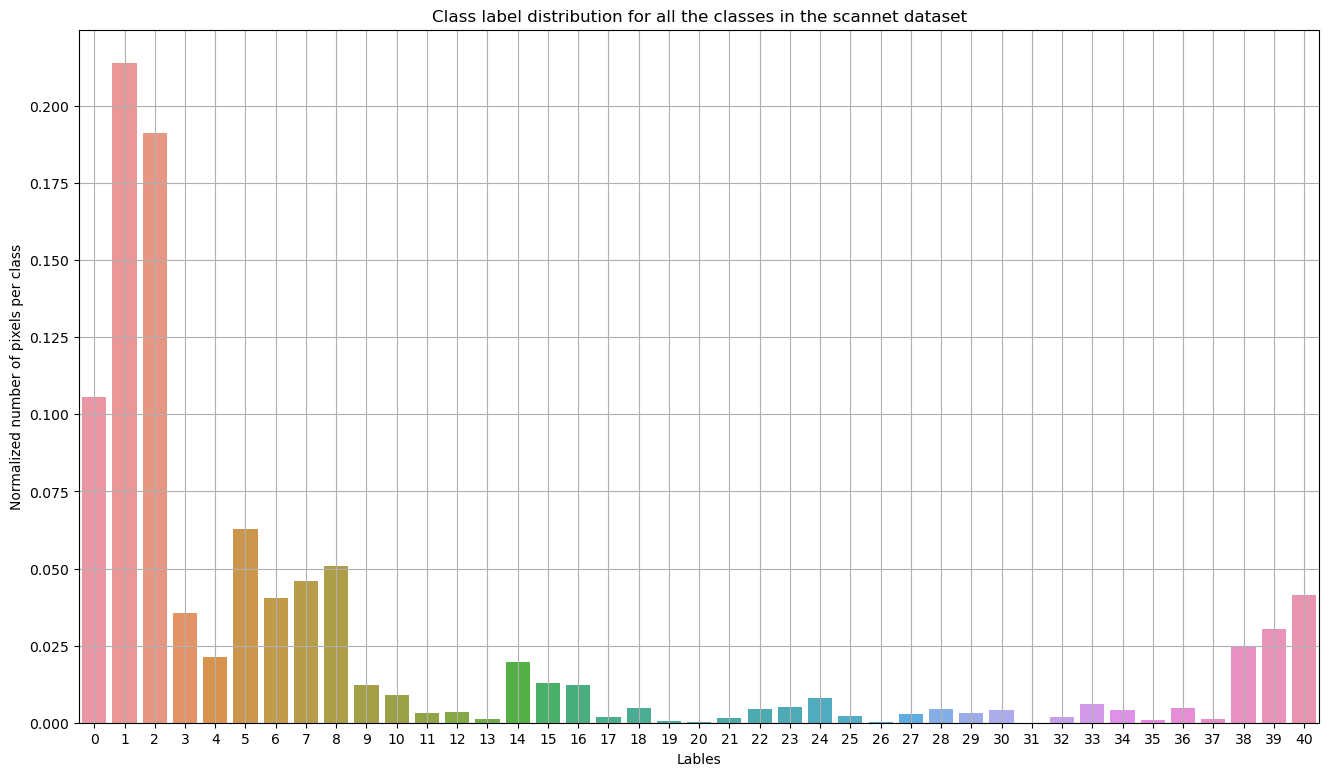
\includegraphics[width=13cm]{images/scannet_data_class_distribution.png}
    	\caption{Per class pixel distribution of the entire scannet dataset}
    	\label{fig:scannet_class}
    \end{figure} 
    
    \begin{figure}%
    	\centering
    	\subfloat[\centering Per class pixel distribution of the training dataset pixel class label ]{{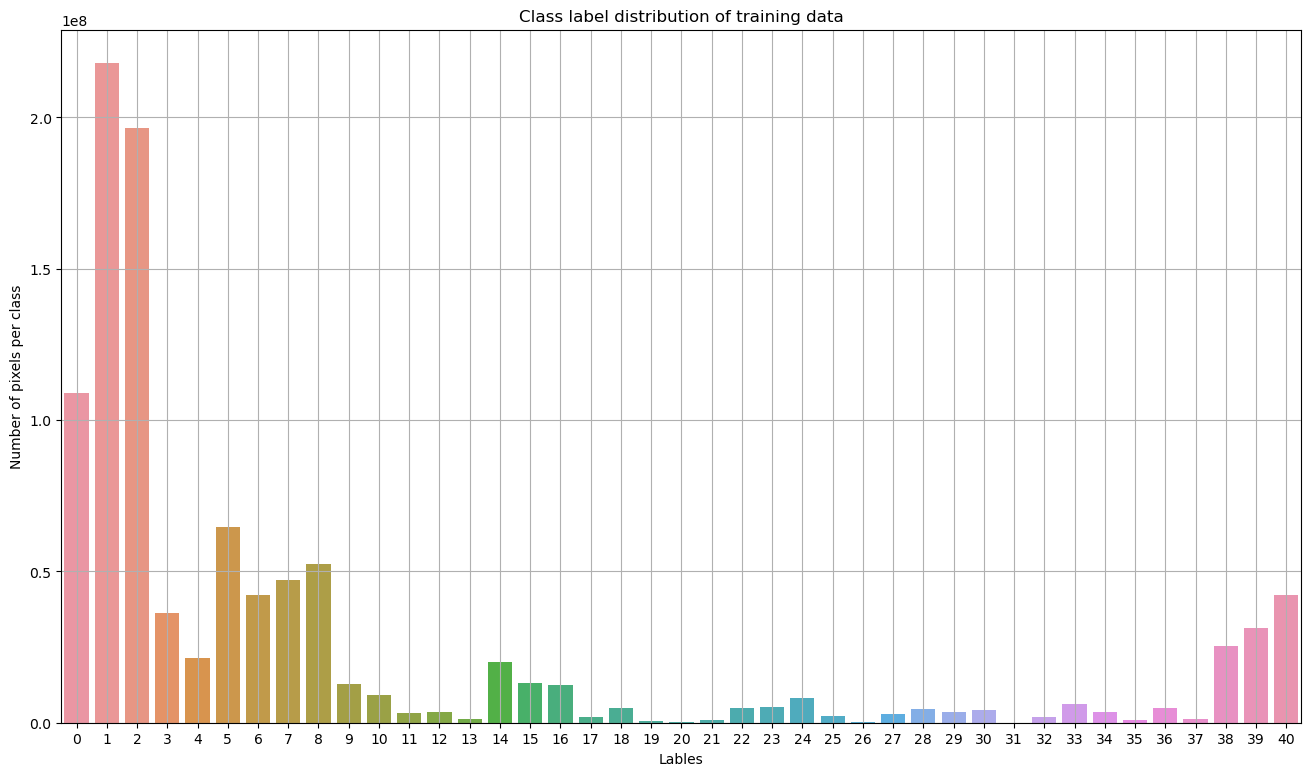
\includegraphics[width=7cm]{images/scannet_training_data_class_distribution.png} }}%
    	\qquad
    	\subfloat[\centering Per class pixel distribution of the testing dataset pixel class label]{{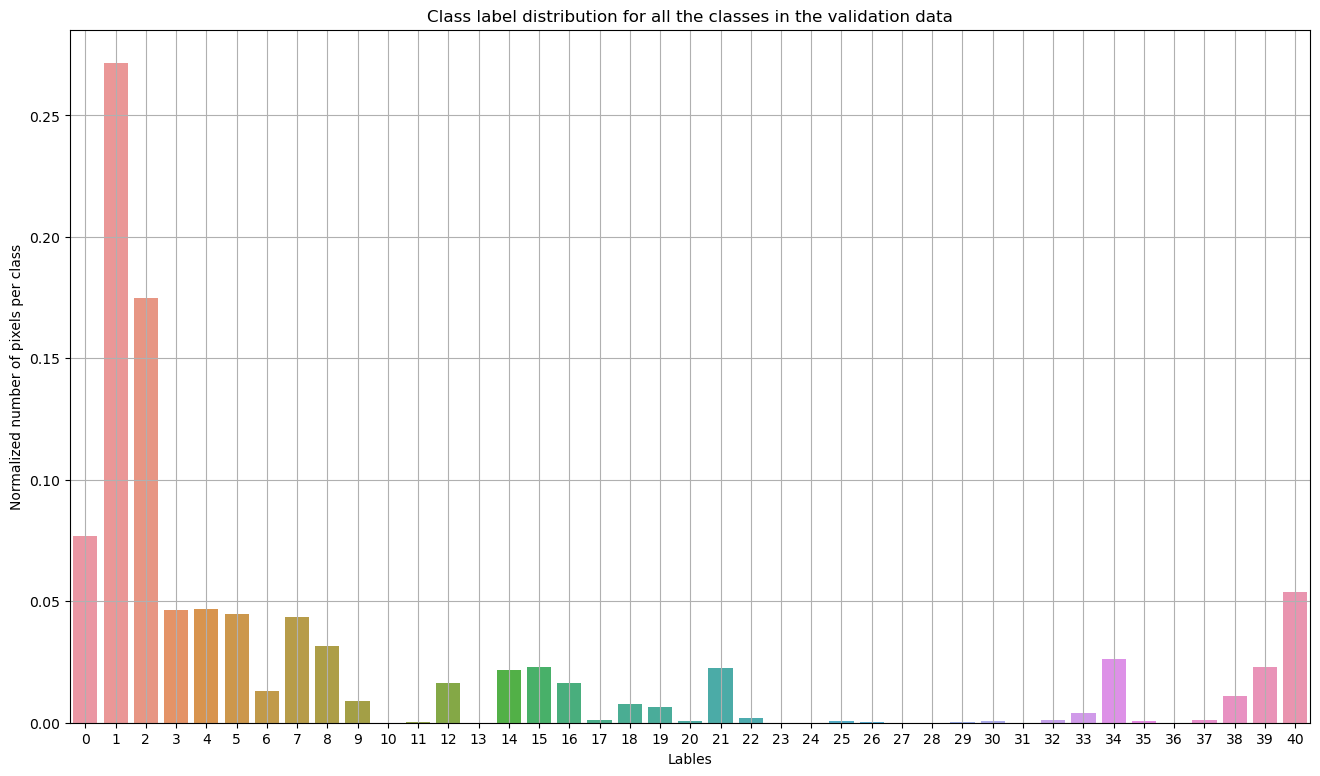
\includegraphics[width=7cm]{images/scannet_testing_data_class_distribution.png} }}%
    	\caption{Pixel distribution for the scannet data containing all the classes}%
    	\label{fig:scannet_all_classes}%
    \end{figure}
    
    \begin{figure}%
    	\centering
    	\subfloat[\centering Per class pixel distribution of the training dataset pixel class label ]{{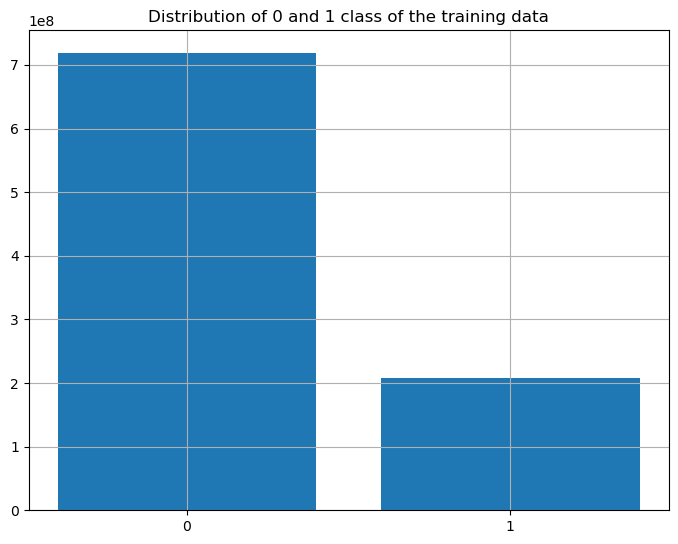
\includegraphics[width=7cm]{images/scannet_training_data_class_distribution_two_classes.png} }}%
    	\qquad
    	\subfloat[\centering Per class pixel distribution of the testing dataset pixel class 	label]{{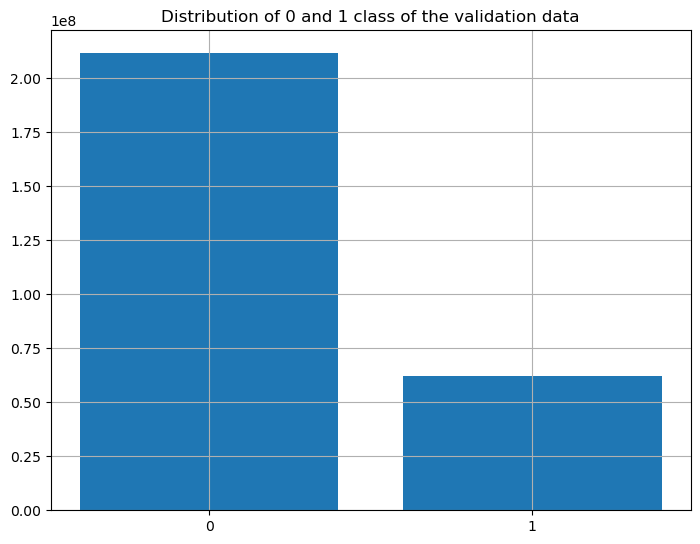
\includegraphics[width=7cm]{images/scannet_testing_data_class_distribution_two_classes.png} }}%
    	\caption{Pixel distribution for the scannet data for two classes}%
    	\label{fig:scannet_two_classes}%
    \end{figure}

   	\begin{figure}%
    	\centering
    	\subfloat[\centering Per class pixel distribution of the training dataset pixel class label ]{{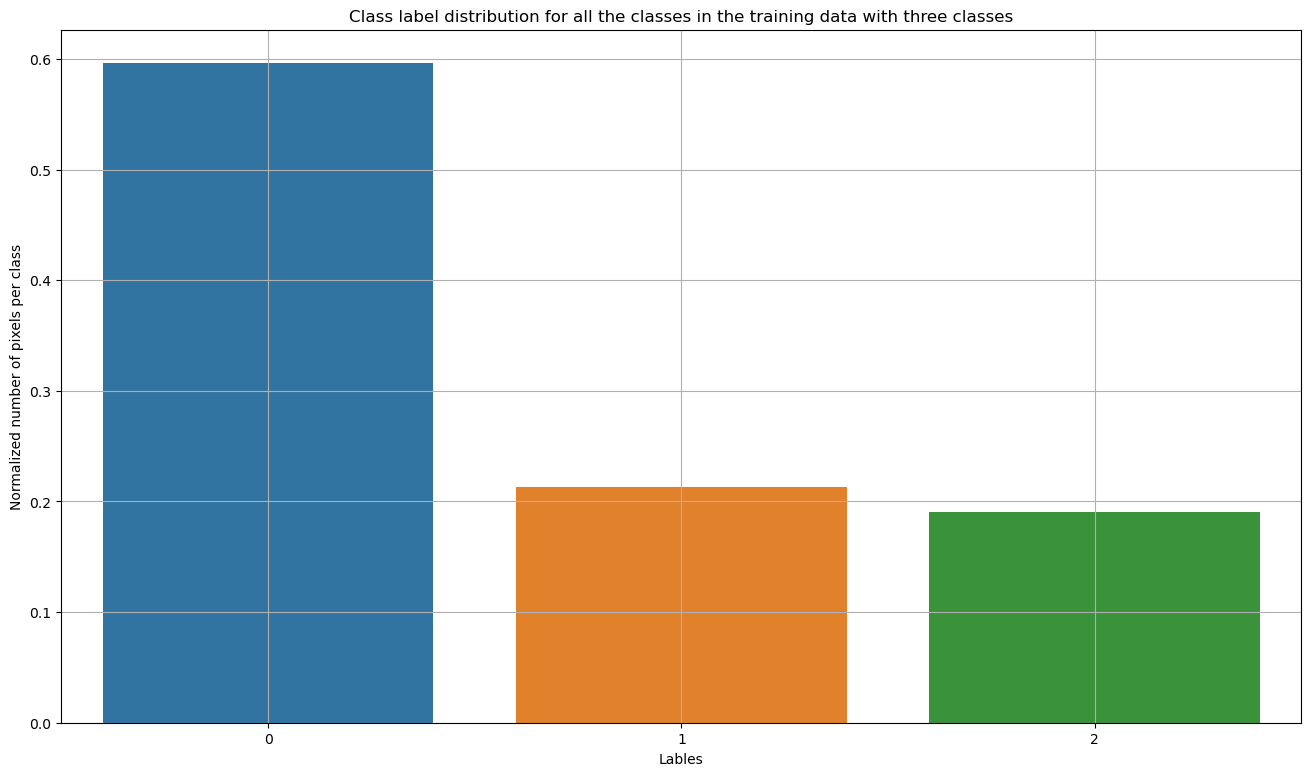
\includegraphics[width=7cm]{images/scannet_training_data_class_distribution_three_classes.png} }}%
    	\qquad
    	\subfloat[\centering Per class pixel distribution of the testing dataset pixel class 	label]{{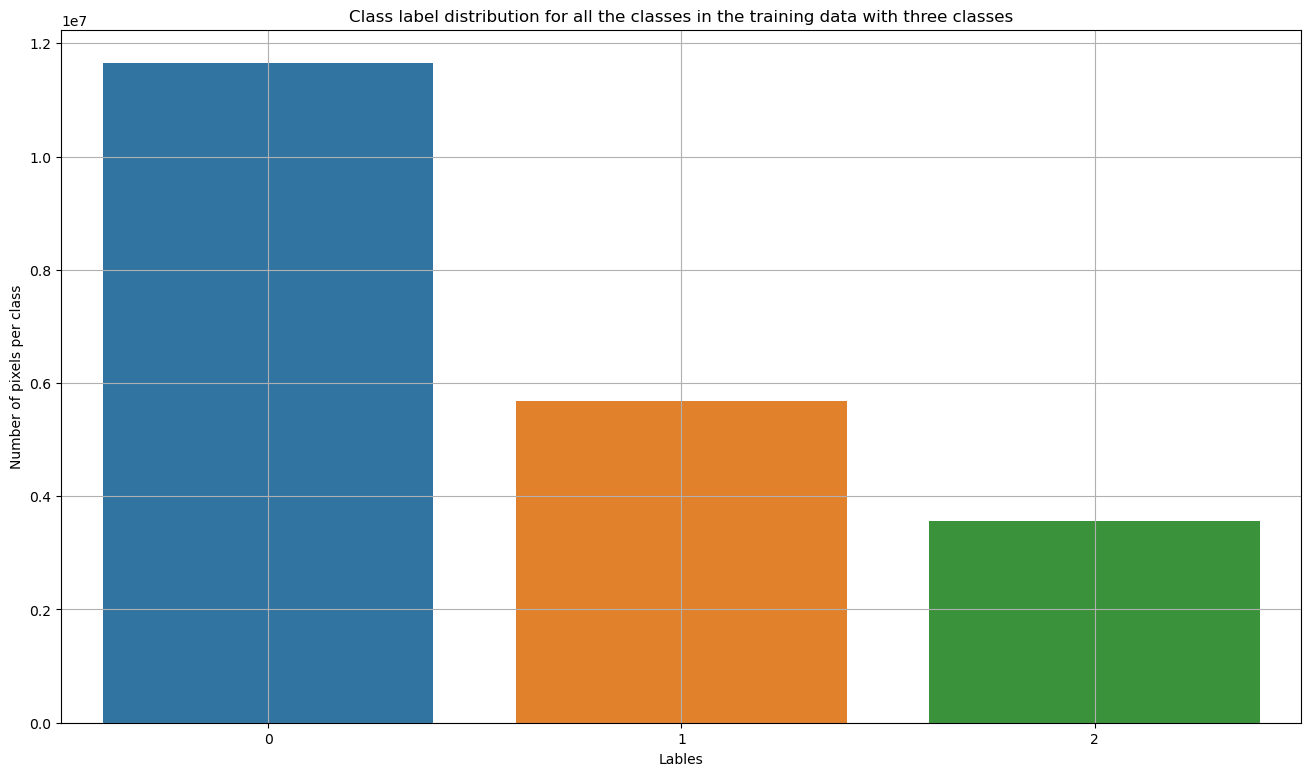
\includegraphics[width=7cm]{images/scannet_testing_data_class_distribution_three_classes.png} }}%
    	\caption{Pixel distribution for the scannet data for three classes}%
    	\label{fig:scannet_three_classes}%
    \end{figure}
    %---------------------------------------------------------------------------------------------------------
    \subsection{Distance and Kernel matrix}
	
	A distance matrix is a square matrix that represent the distance between the pair of objects. Distance matrix can be constructed from the pose information of the captured video sequence. Closer the two frames are in a sequence the distance between them is smaller, same can be represented with the matrix plot. Two types of distance matrix is plotted in the Fig \ref{fig:ordered_D_and_K} and \ref{fig:unordered_D_and_K}. In the first type of plot, a ordered frames pose is represented in the x and y axis. The distance of pose with respect to itself is zero and as the frame number is increased the distance keeps increasing. In the second type of unordered pose plot the frames pose are shuffled and presented as the matrix plot. These pictures represent the distance of one frame to the other. 
	
	\begin{figure}[h]
		\centering
		\subfloat[\centering Ordered set of images]{{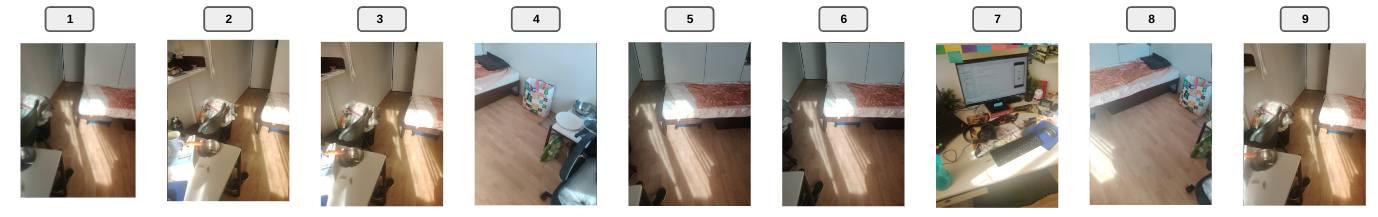
\includegraphics[width=14cm]{images/ordered_images.jpg} }}%
		\qquad
		\subfloat[\centering Unordered set of images label]{{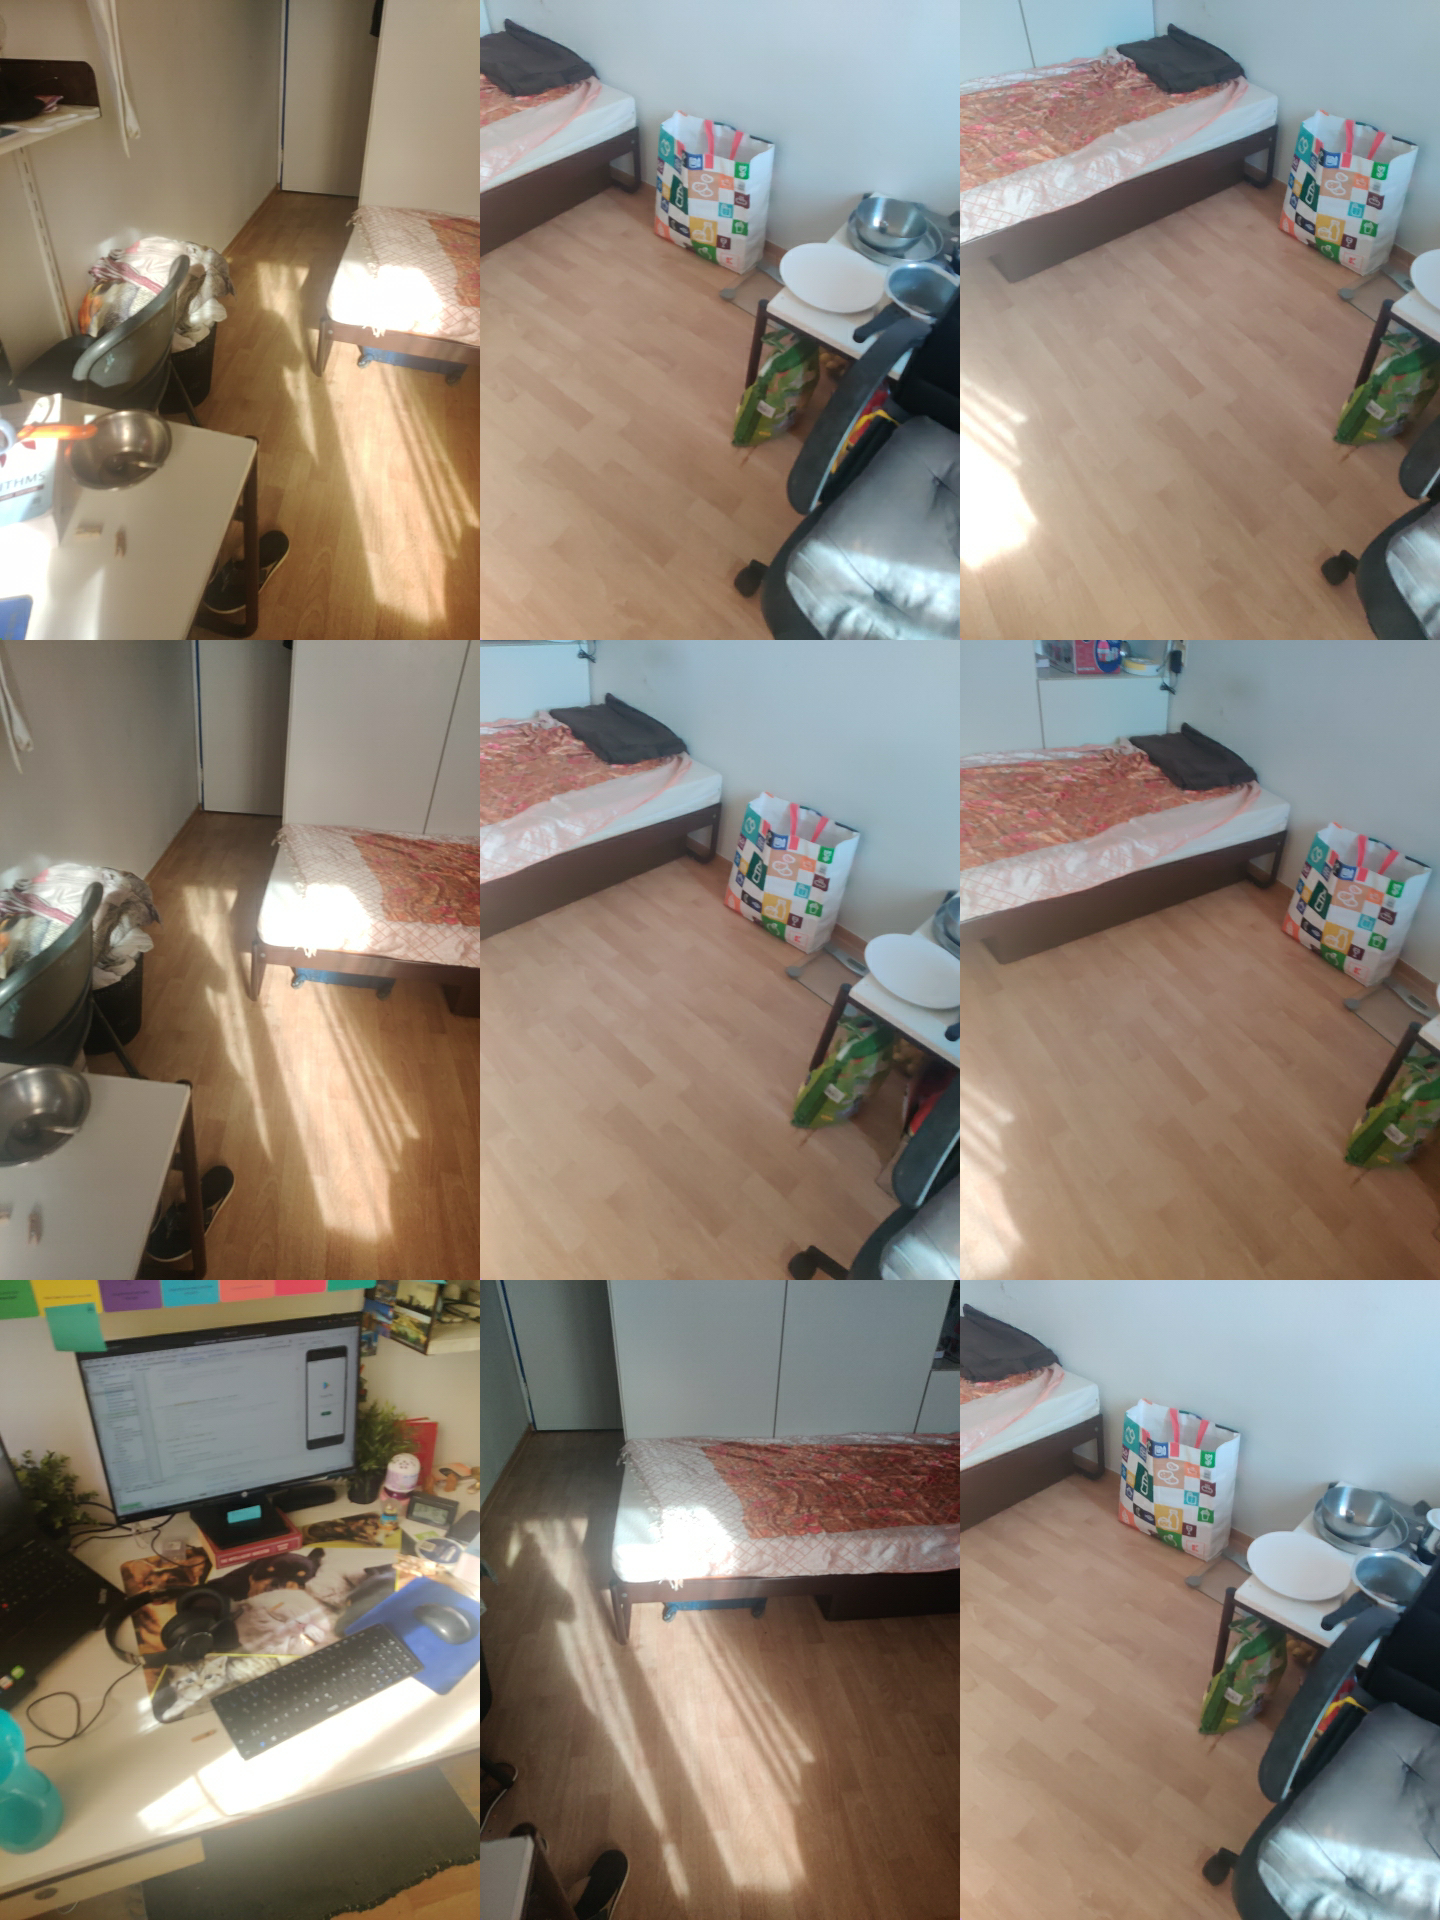
\includegraphics[width=14cm]{images/unordered_images.jpg} }}%
		\caption{Ordered and Unordered set of images}%
		\label{fig:ordered_and_unordered_images}%
	\end{figure}
	
	The distance matrix is used to construct the kernel of the Gaussian process. Kernel represent the similarity or correlation between the two data points. Closer data points in the distance space have high correlation and further away data points have low correlation, and same can be observed in the plotting of the kernal matrix as heatmap in Fig \ref{fig:ordered_D_and_K} and \ref{fig:unordered_D_and_K}. The corresponding ordered and unordered frames images are presented in \ref{fig:ordered_and_unordered_images}.  
	
	\begin{figure}
		\centering
		\subfloat[\centering Distance matrix depicted as heatmap ]{{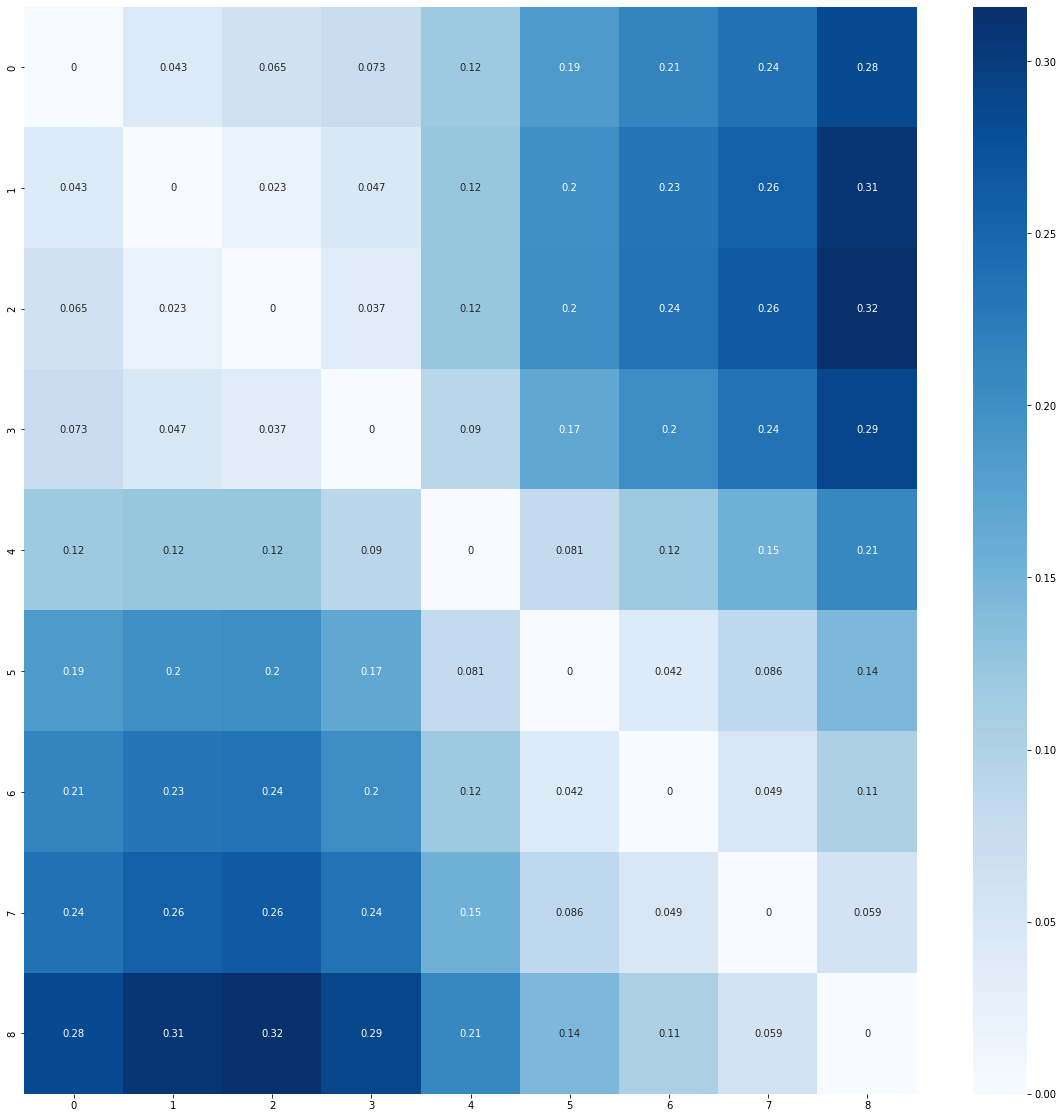
\includegraphics[width=7cm]{images/ordered_D.png} }}%
		\qquad
		\subfloat[\centering Kernel matrix depicted as heatmap label]{{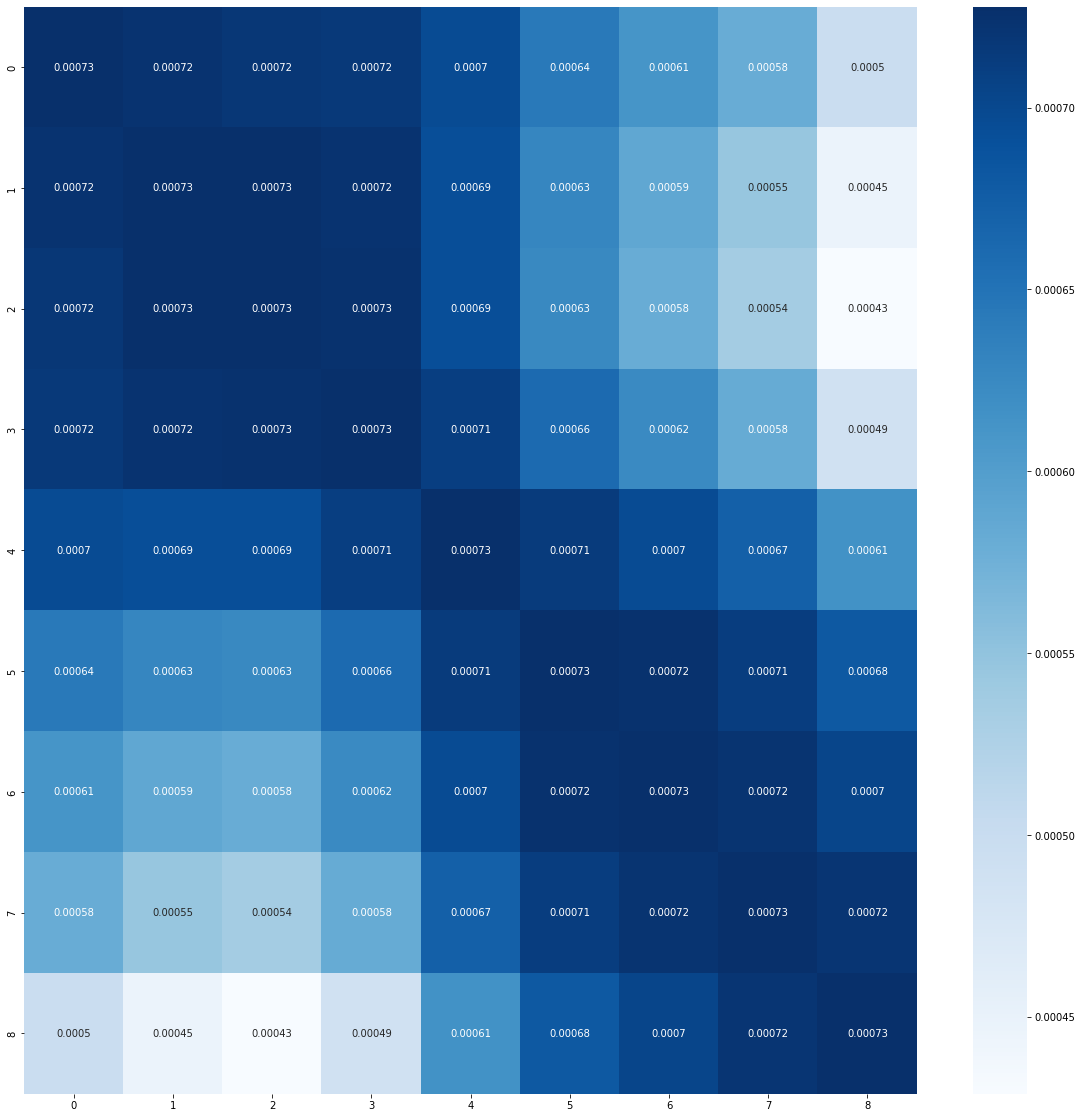
\includegraphics[width=7cm]{images/ordered_K.png} }}%
		\caption{Distance matrix and Kernel matrix for ordered set of images}%
		\label{fig:ordered_D_and_K}%
	\end{figure}
	
	\begin{figure}
		\centering
		\subfloat[\centering Distance matrix depicted as heatmap ]{{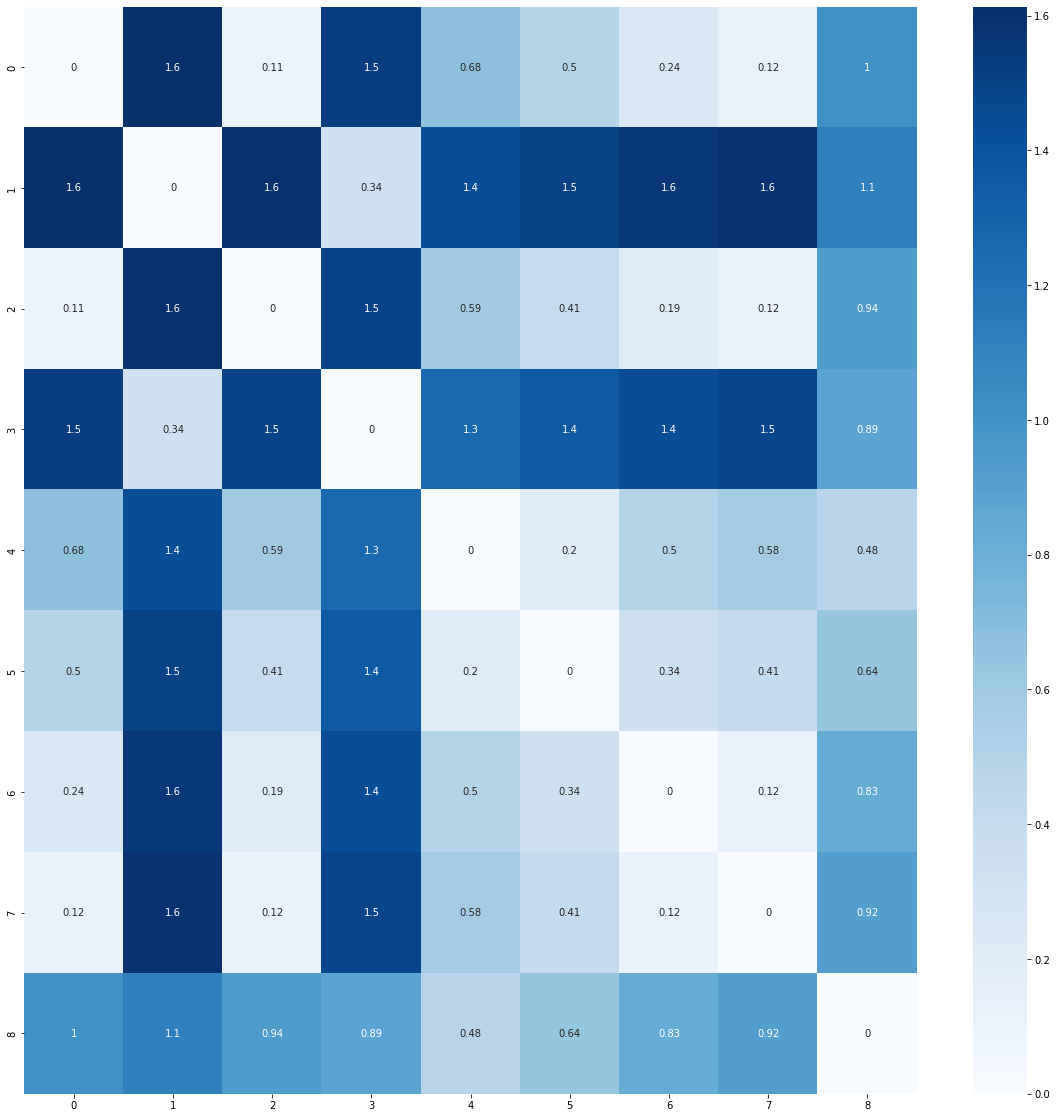
\includegraphics[width=7cm]{images/unordered_D.png} }}%
		\qquad
		\subfloat[\centering Kernel matrix depicted as heatmap 	label]{{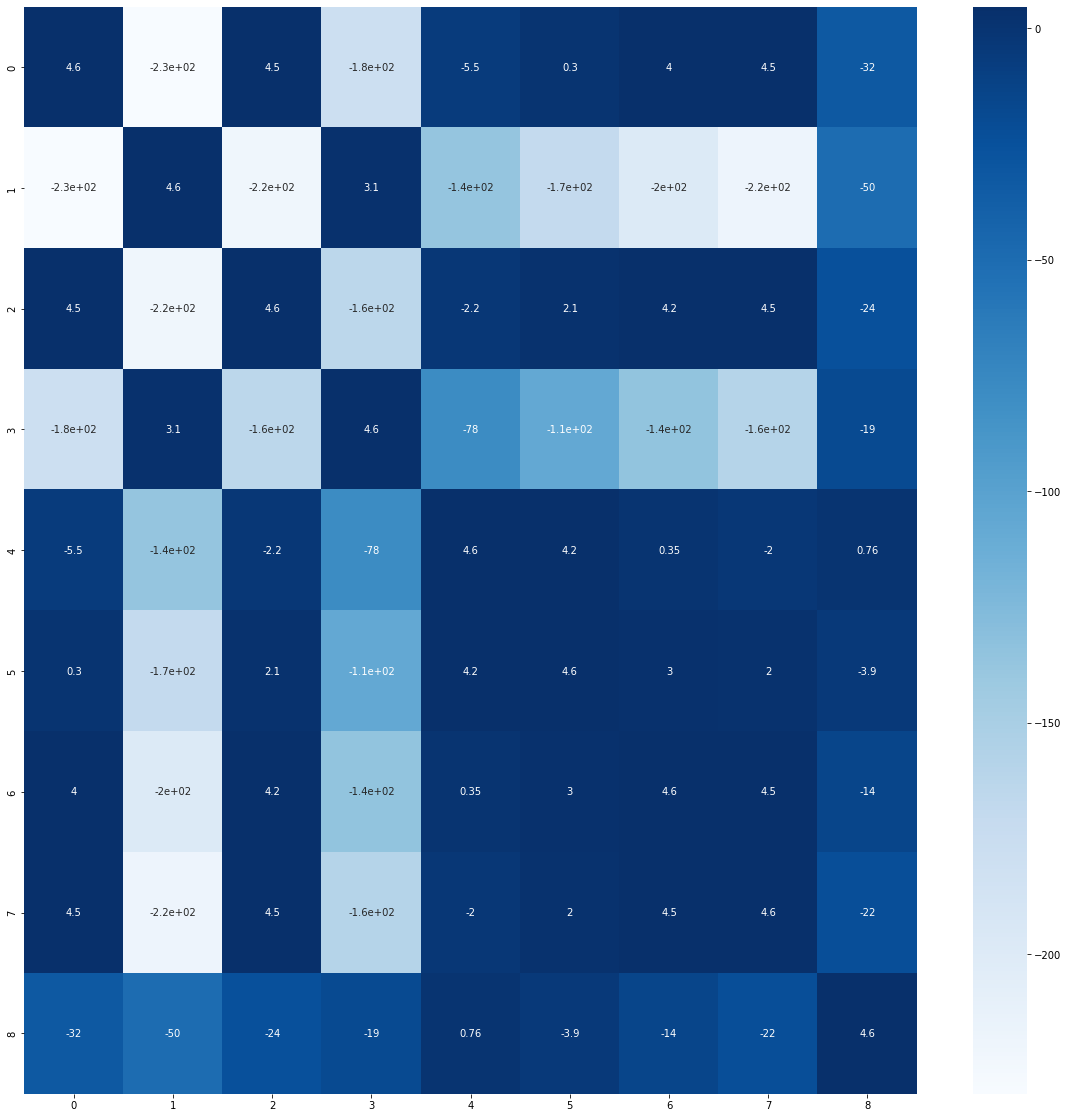
\includegraphics[width=7cm]{images/unordered_K.png} }}%
		\caption{Distance matrix and Kernel matrix for unordered set of images}%
		\label{fig:unordered_D_and_K}%
	\end{figure}
	
	%---------------------------------------------------------------------------------------------------------

    \subsection{Experiment1.1: U-Net Vanilla, GP and LSTM model considering all the classes}
    
    Below sections explains the results of the conducted experiments. The model is trained and tested with the scannet dataset without merging the classes. The models performance is evaluated with Pixel accuracy, Mean pixel accuracy, meanIoU, IoU and FwIoU metrics.
    
    %{ \bf Experiment1.1.1: U-Net vanilla model with all the classes}
    { \bf Experiment1.1.2: U-Net vanilla model}
    
    The pixel accuracy is 50.96\% for the validation dataset. The is due to the presence of large number of classes with unequal pixel distribution. However, the IoU for the Wall, Floor and Mattress is high at 0.56, 0.608, 0.382 due to the high pixel distribution for these classes. Frequency weighted IoU take into account the unequal pixel distribution and the values stand at 0.3531. The predicted and the ground truth pixel distribution is presented in the Fig \ref{fig:y_gt_pred_vanilla}. From the bar plot it is evident that predicted "Wall" class distribution is high compared to the ground truth. The Wall and Floor class distribution is similar as the baseline and predicted class labels. 
    
    %------------------------------------------------------------------------------------------------------
   	
   	\begin{table}
    \begin{center}
    	\begin{tabular}{ | l | p{12cm} |}
    		\hline
    		
    		\cellcolor{purple!30}Metric & \cellcolor{purple!30}Value \\ \hline
    		Pixel Accuracy & 0.5096 \\ \hline
    		Pixel Mean accuracy & 0.1907  \\ \hline
    		meanIOU & 0.1102 \\ \hline
    		IoU & [1.8345e-01, 5.6047e-01, 6.0881e-01, 1.6476e-01, 3.8241e-01, 1.1697e-01, 
    		2.3122e-02, 8.9410e-02, 2.5848e-01, 1.6661e-01, 2.0180e-03, 2.0504e-01, 
    		4.5985e-02,        nan, 4.2167e-02, 1.1143e-01, 2.3969e-01, 1.2545e-02, 
    		1.1324e-01, 2.7658e-03, 0.0000e+00, 7.0415e-02, 7.0606e-02, 0.0000e+00,  
    		0.0000e+00, 1.2208e-01, 1.4680e-02, 1.1862e-04, 2.2112e-04, 6.5610e-03, 
    		4.3742e-03,        nan, 7.6680e-02, 3.5784e-02, 1.1516e-01, 5.6912e-02, 
    		2.9310e-04, 3.7764e-02, 2.2634e-02, 1.1269e-01, 2.2094e-01] \\ \hline
    		FwIoU & 0.3531 \\ \hline
    		\hline
    	\end{tabular}
   		\caption{A normal caption}
	    \label{tab:caption}
    \end{center}
	\end{table}

	\begin{figure}%
		\centering
		\subfloat[\centering Per class pixel distribution of the ground truth pixel class label ]{{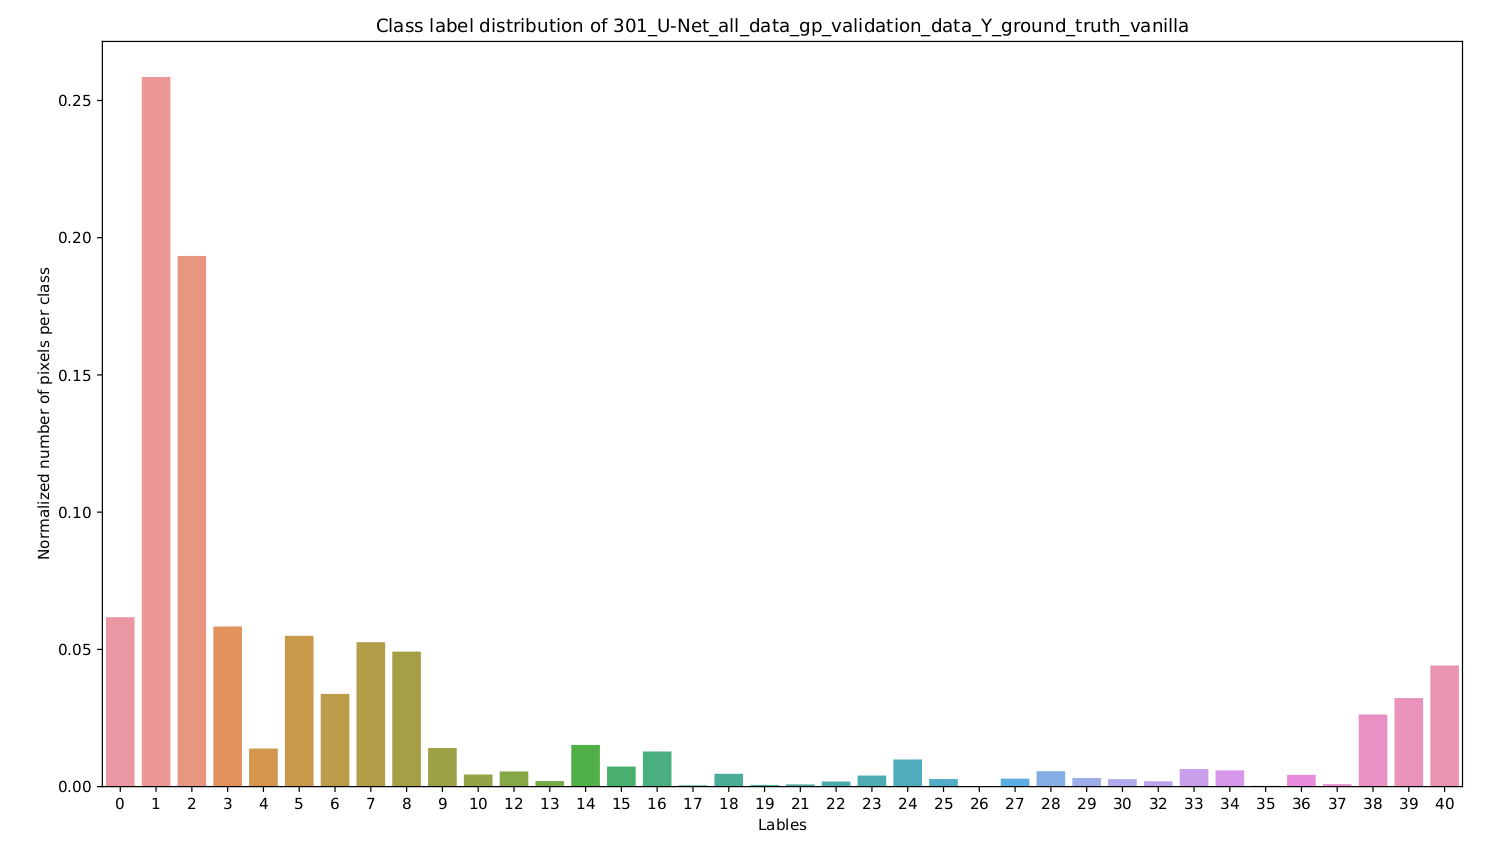
\includegraphics[width=7cm]{images/Y_ground_truth_vanilla.png} }}%
		\qquad
		\subfloat[\centering Per class pixel distribution of the predicted pixel class label]{{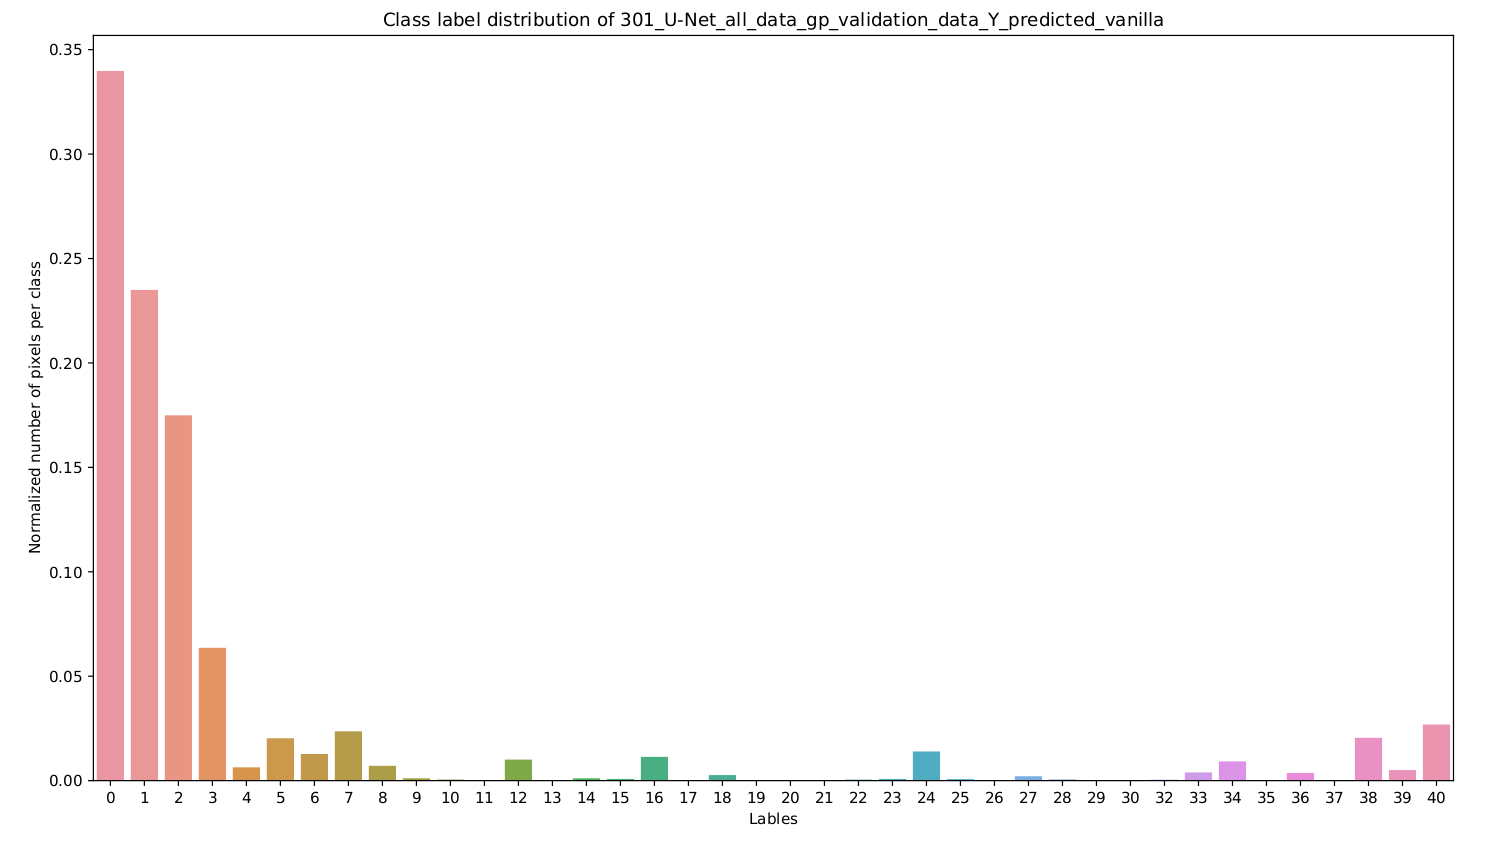
\includegraphics[width=7cm]{images/Y_predicted_vanilla.png} }}%
		\caption{Pixel distribution for the ground truth and predicted scannet data for vanilla unet model}%
		\label{fig:y_gt_pred_vanilla}%
	\end{figure}
    %------------------------------------------------------------------------------------------------------
    { \bf Experiment1.1.2: U-Net gp model}
    
    In the gp model experiment the information from the previous frame is passed onto the current frame segmentation computation. The accuracy is slightly better than the vanilla model with a increase of 1\% with the temporal fusion GP prior integration. The latent space encoding is subjected to the Gaussian process and then passed onto the decoder for segmentation computation. The mean pixel accuracy is similar to the vanilla model with not much improvements. The presence of large number of classes is causing the drop in the performance. As expected "Wall", "Floor", and "Furniture" class have high IoU values due to the presence of high pixel distribution. 
    
    \begin{table}
	\begin{center}
		\begin{tabular}{ | l | p{12cm} |}
			\hline
			
			\cellcolor{purple!30}Metric & \cellcolor{purple!30}Value \\ \hline
			Pixel Accuracy & 0.5184 \\ \hline
			Pixel Mean accuracy & 0.1679  \\ \hline
			meanIOU & 0.1161 \\ \hline
			IoU & [1.7087e-01, 5.1271e-01, 5.9998e-01, 2.1256e-01, 4.1160e-01, 1.5834e-01,
			3.8634e-02, 2.3669e-01, 1.6056e-01, 1.1568e-01, 7.9677e-02, 1.0454e-02,
			2.4003e-02, 0.0000e+00, 1.2199e-01, 4.3193e-02, 3.3956e-01, 6.6473e-02,
			1.4712e-01, 2.8003e-03, 6.0475e-05, 2.6127e-01, 5.7962e-02, 0.0000e+00,
			3.4611e-04, 1.6519e-02, 0.0000e+00, 4.3417e-04, 4.4221e-02, 6.6478e-03,
			1.2108e-02,        nan, 5.3272e-02, 5.8480e-02, 2.2352e-01, 4.2175e-02,
			8.4644e-02, 1.1630e-04, 4.9106e-02, 1.0338e-01, 1.7687e-01] \\ \hline
			FwIoU & 0.3497 \\ \hline
			\hline
		\end{tabular}
		\caption{A normal caption}
		\label{tab:caption}
	\end{center}
	\end{table}
	
	\begin{figure}%
		\centering
		\subfloat[\centering Per class pixel distribution of the ground truth pixel class label for gp model ]{{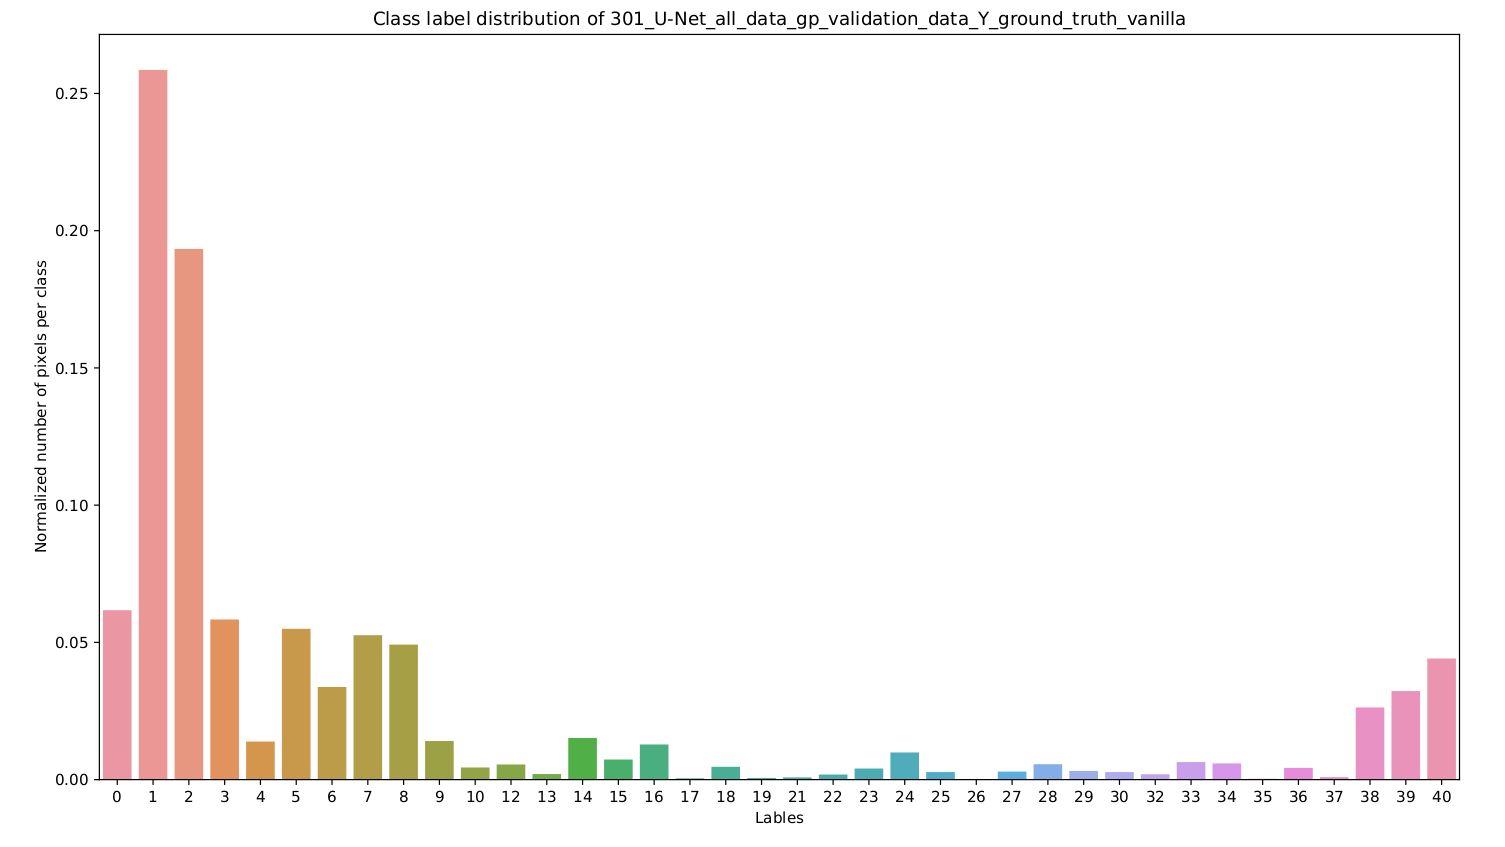
\includegraphics[width=7cm]{images/Y_ground_truth_gp.png} }}%
		\qquad
		\subfloat[\centering Kernel matrix depicted as heatmap 	label]{{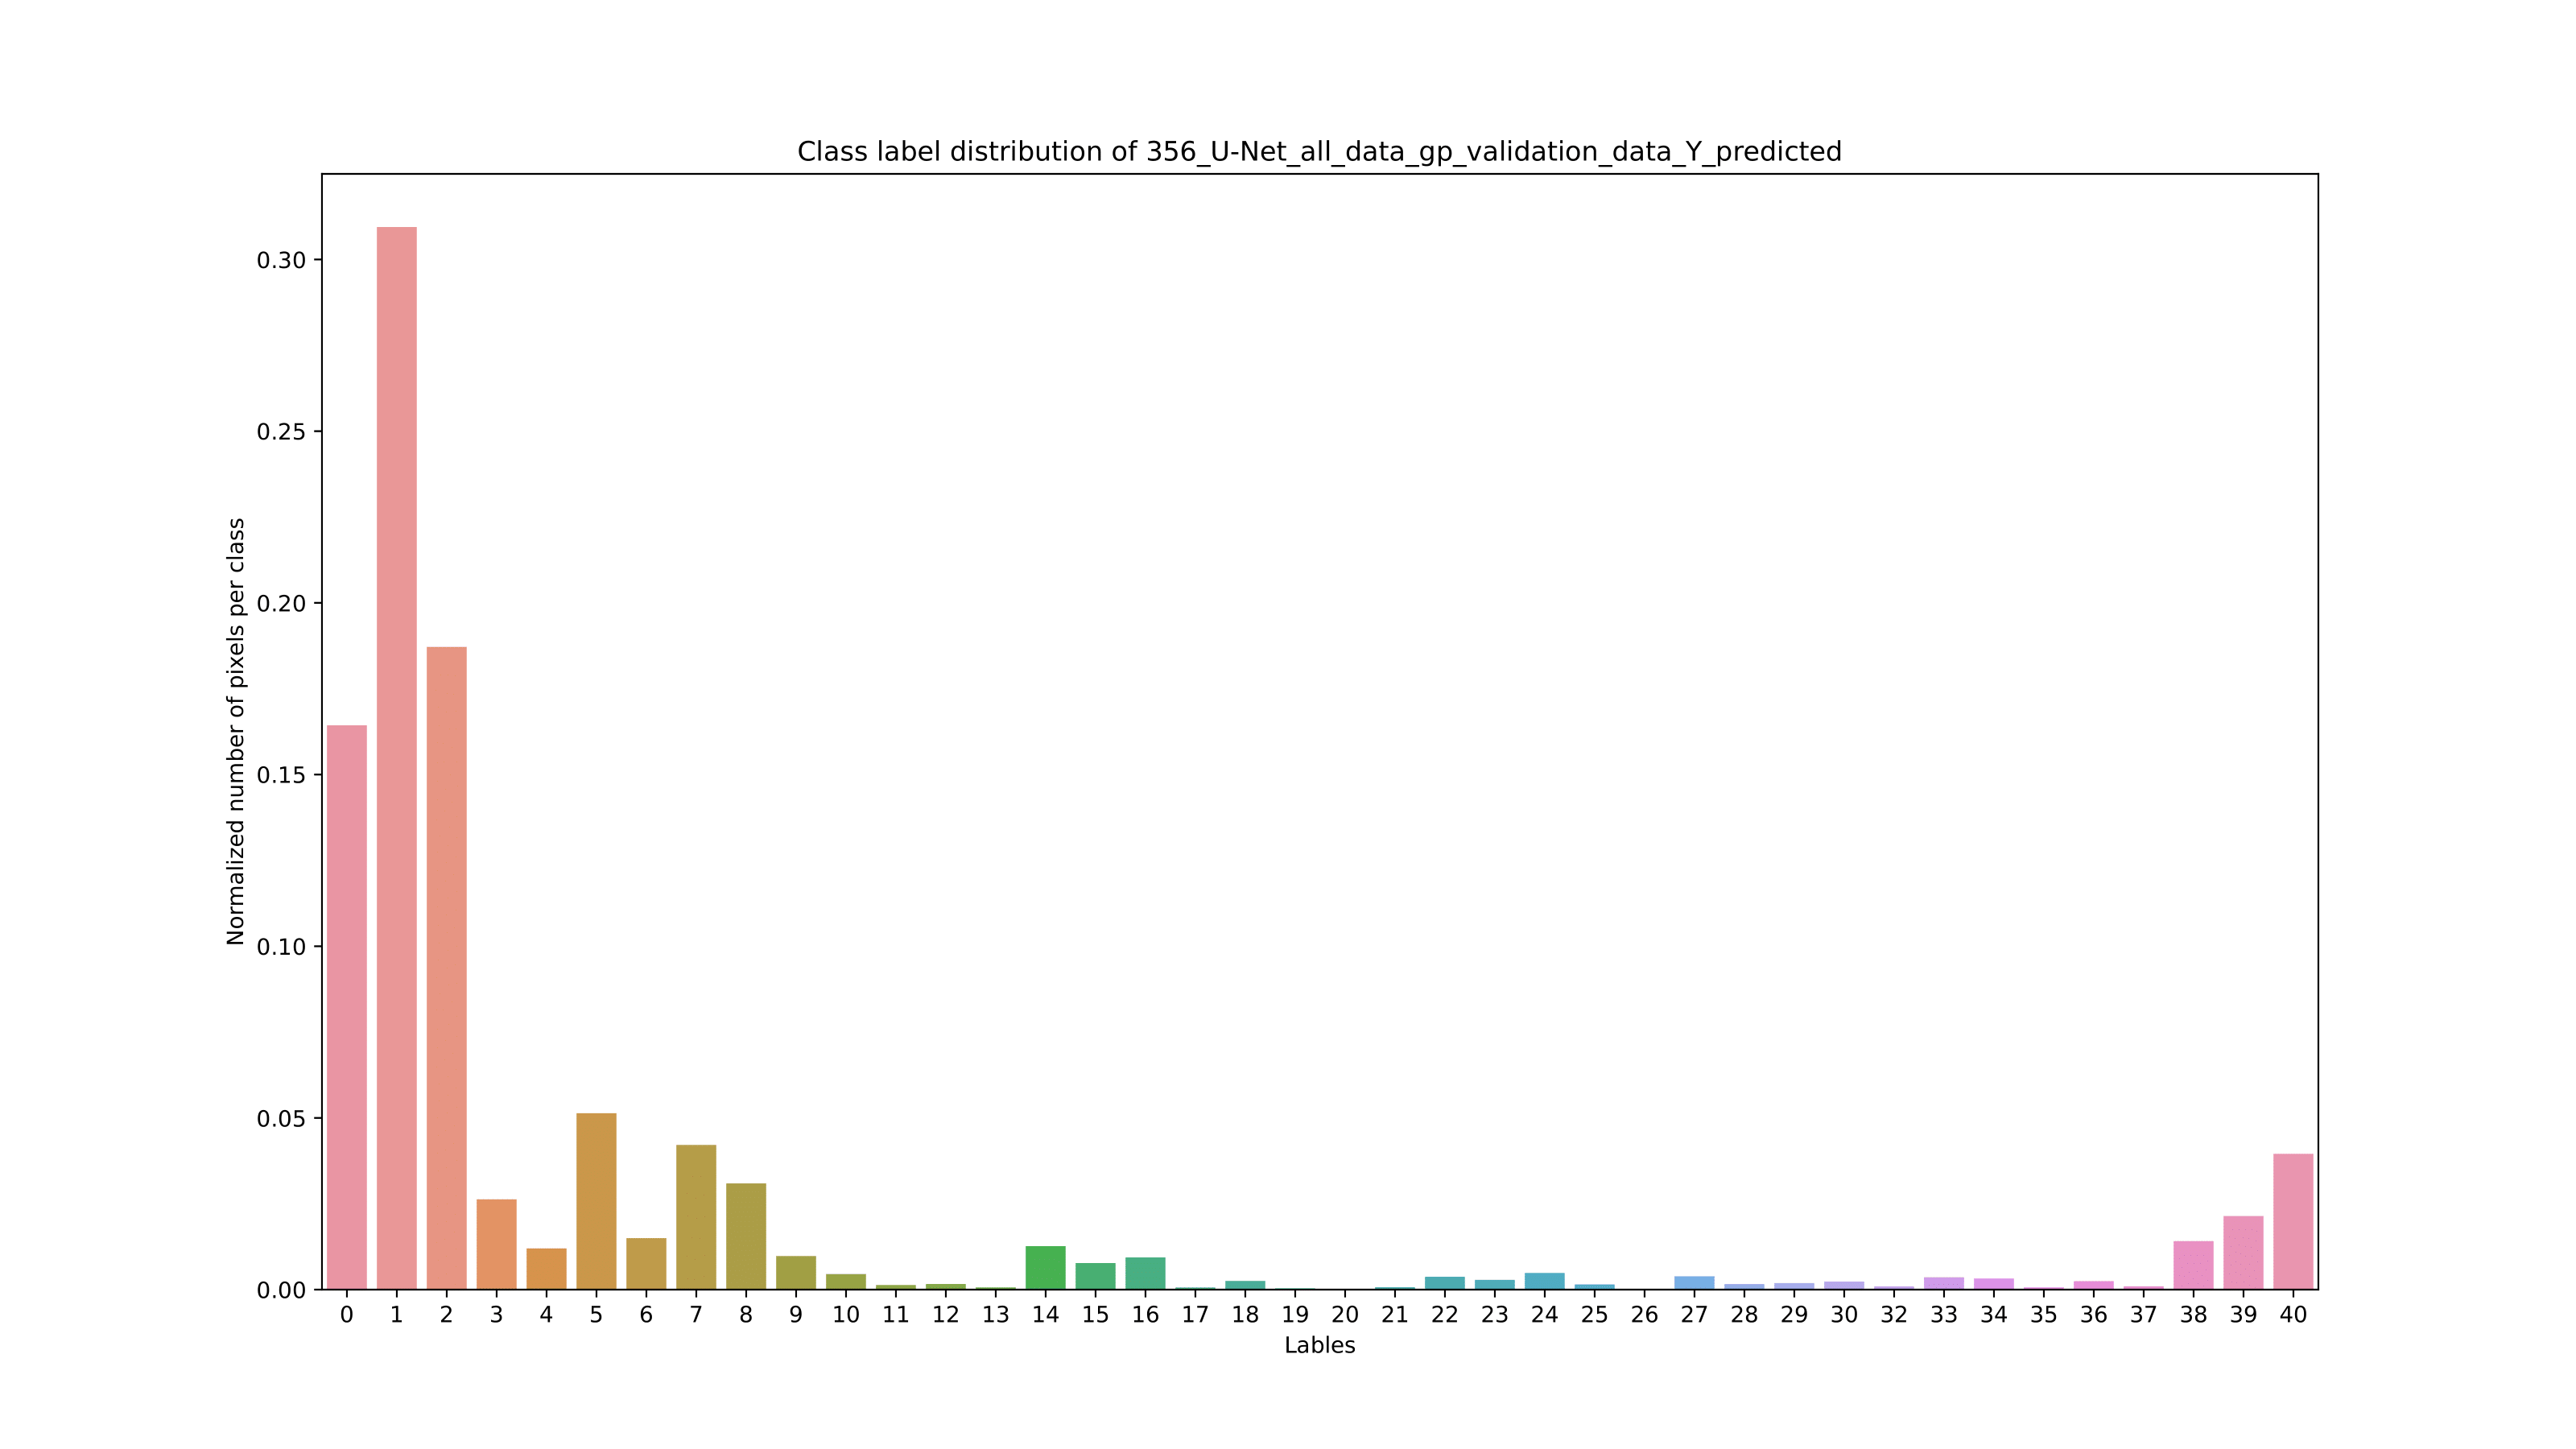
\includegraphics[width=7cm]{images/Y_predicted_gp.png} }}%
		\caption{Per class pixel distribution of the predicted pixel class label for gp model}%
		\label{fig:y_gt_and_predic_gp}%
	\end{figure}

    %------------------------------------------------------------------------------------------------------
    \newpage
	{ \bf Experiment1.1.2: U-Net lstm model}
	
	The scene geometry from the past frame is passed onto a current frame in a efficient manner with the lstm model. The ConvLSTM cell at the latent space compress and store the past information in its states. The change in the viewpoint is captured by the hidden state and passed onto the next hidden state for the computation of the segmentation map. From the result table \ref{tab:lstm_result_all_classes} it is evident that the accuracy has improved by 6\% and 5\% in comparison with the vanilla and gp models respectively. Mean accuracy has increased by a quite a big margin. The IoU values are also improved by a large margin. IoU for the "Wall" class is highest with 0.61 in comparison with vanilla and gp approach. However, for the cabinet class gp performed well. Table, bookshelf, Counter, desk class gp outperformed the vanilla and lstm model. 
	
	\begin{table}
	\begin{center}
		\begin{tabular}{ | l | p{12cm} |}
			\hline		
			\cellcolor{purple!30}Metric & \cellcolor{purple!30}Value \\ \hline
			Pixel Accuracy & 0.5426 \\ \hline
			Pixel Mean accuracy & 0.3509  \\ \hline
			meanIOU & 0.1411 \\ \hline
			IoU & [0.1690, 0.5573, 0.5949, 0.1428, 0.1170, 0.1984, 0.1930, 0.1278, 0.2010,
			0.0778, 0.0071, 0.0514, 0.0216, 0.0070, 0.0426, 0.0610, 0.1063, 0.0020,
			0.0907, 0.0017, 0.0000, 0.0114, 0.0422, 0.0015, 0.0380, 0.0209, 0.0000,
			0.0362, 0.0710, 0.0010, 0.0182, 0.0000, 0.0174, 0.1382, 0.0534, 0.0077,
			0.0558, 0.0016, 0.0646, 0.1776, 0.1697] \\ \hline
			FwIoU & 0.7643 \\ \hline
			\hline
		\end{tabular}
		\caption{A normal caption}
		\label{tab:caption}
	\end{center}
	\end{table}
	
	\begin{figure}%
		\centering
		\subfloat[\centering Per class pixel distribution of the ground truth pixel class label for lstm model ]{{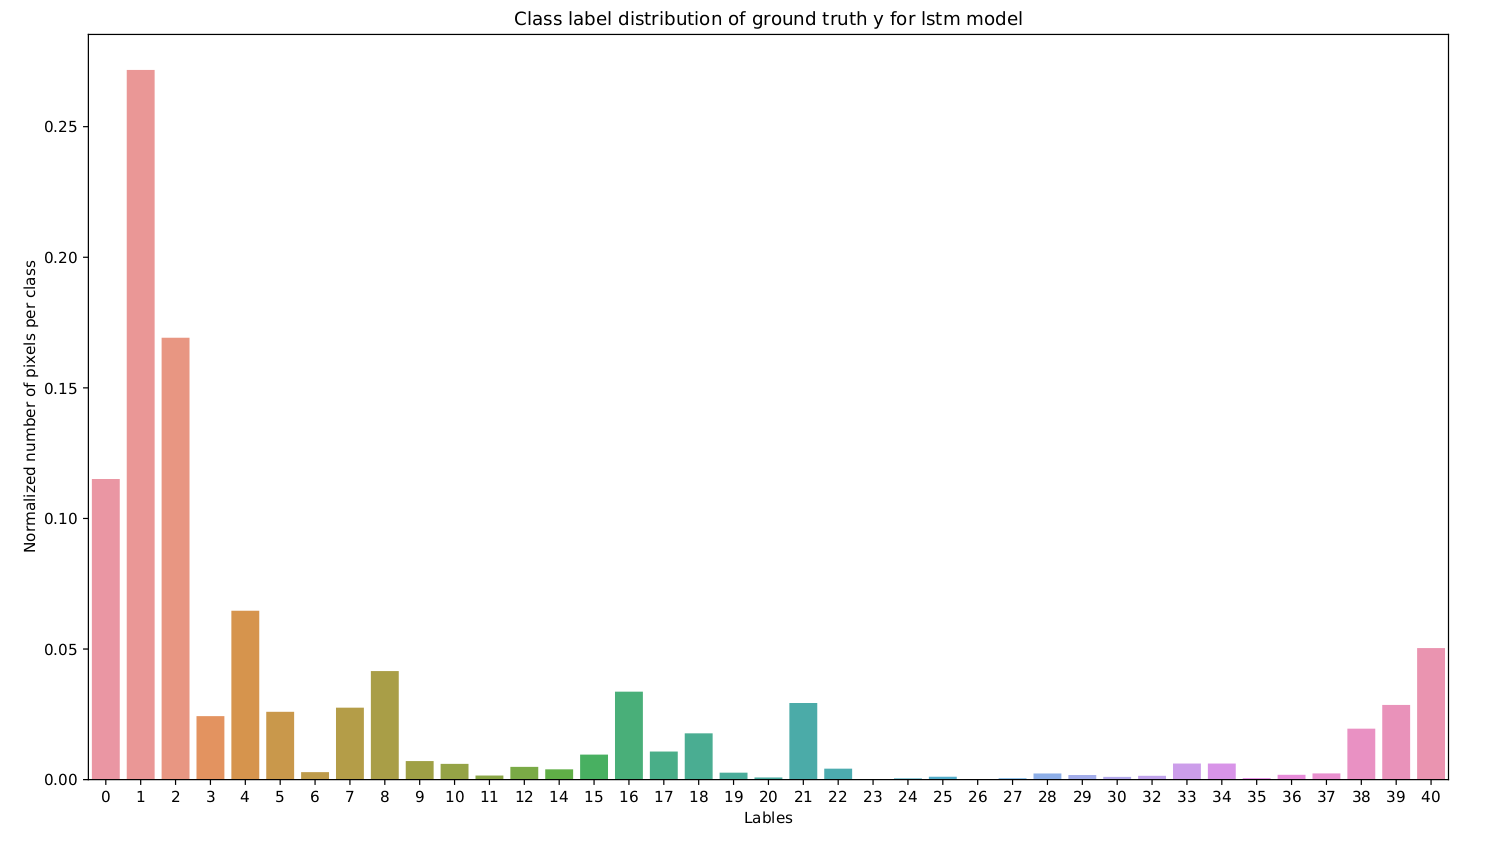
\includegraphics[width=7cm]{images/Y_ground_truth_lstm.png} }}%
		\qquad
		\subfloat[\centering Kernel matrix depicted as heatmap 	label]{{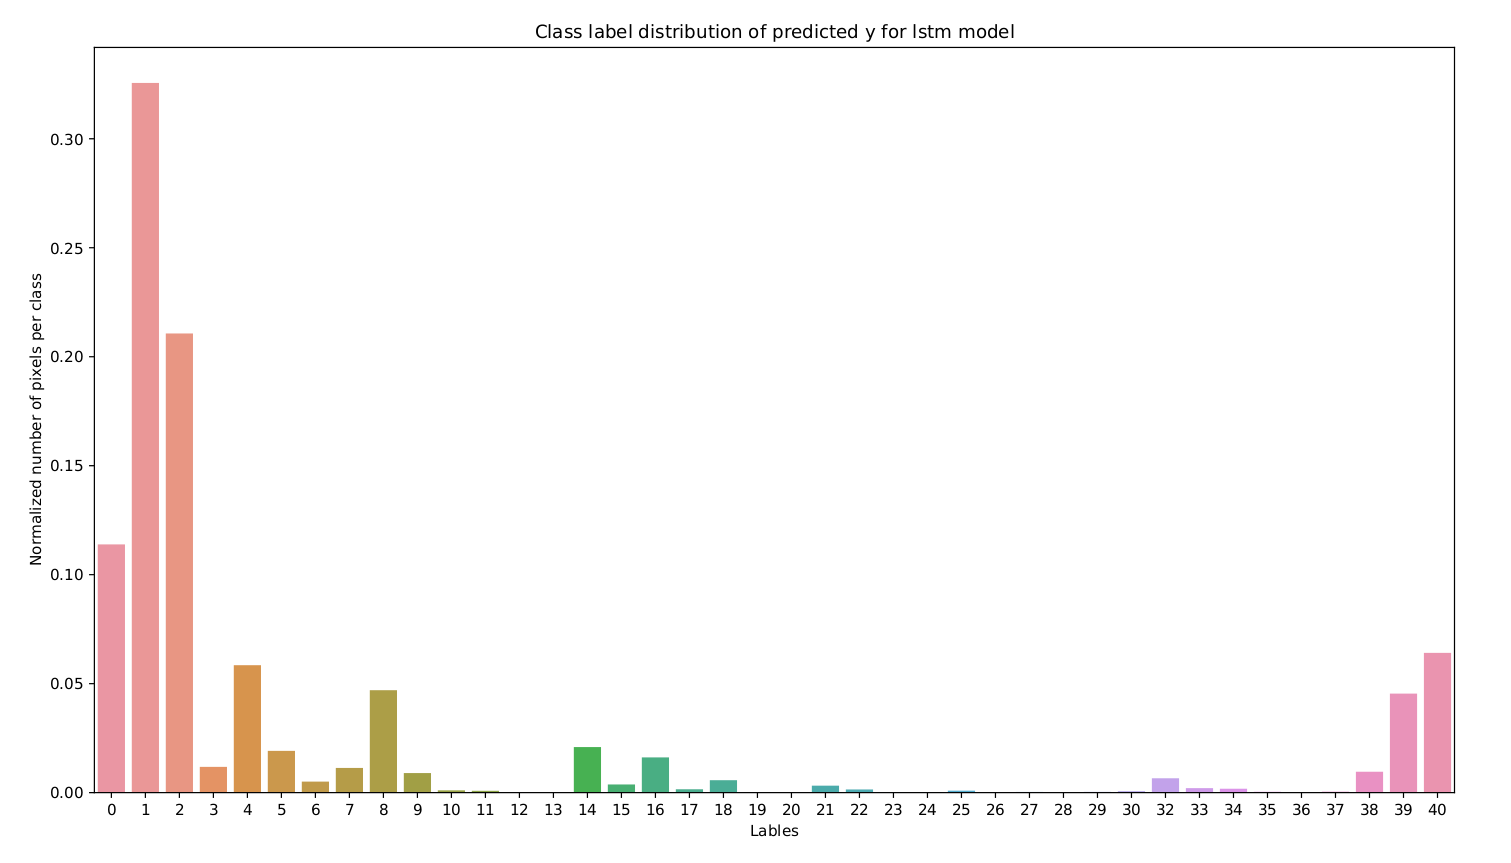
\includegraphics[width=7cm]{images/Y_predicted_lstm.png} }}%
		\caption{Per class pixel distribution of the predicted pixel class label for lstm model}%
		\label{fig:y_gt_and_predic_lstm}%
	\end{figure}

	Accuracy, meanaccuracy, meanIoU, FWIoU comparison is plotted as the bar graph in \ref{fig:unet_model_metric_comparison_all_classes}. The accuracy is highest for the lstm model in comparison with the vanilla and gp. However, the mean accuracy is lowest for the gp model with respect to other models. It is evident from the experiment that by incorporating the temporal fusion in the semantic segmentation for the continuous sequence data the performance improves. The overlapping and the past information are learned, stored and passed onto to the computation of the future frames semantic segmentation. The temporal dependency between the frames are exploited to efficiently perform the segmentation by taking pose into account in Gaussian process and compressed information in the hidden state of the ConVlstm cell. The Gaussian process works in the fact that if the two frames are very close to each other, represented by the pose information, there is a high probability of overlapping regions in the consecutive frames. Output of the decoder is based on the input to the decoder. The output of the encoder is passed onto the gaussian process, it takes into account the current and previous pose information and outputs a latent encoding based on the distance between the current and the previous frame. Hence, if two frames are close to each other then the latent output of the Gaussian process are similar resulting in information transfer from the past learnt latent representation to the current latent output resulting in improved performance. The comparison of the raw RGB, ground truth and predicted segmentation map is shown in Fig \ref{fig:unet_model}. It can be observed from the figure that Vanilla and LSTM model performed reasonably well in comparison with the GP model. However, overall metric wise LSTM out performed vanilla and gp.   
	
	\begin{figure}
		\centering
		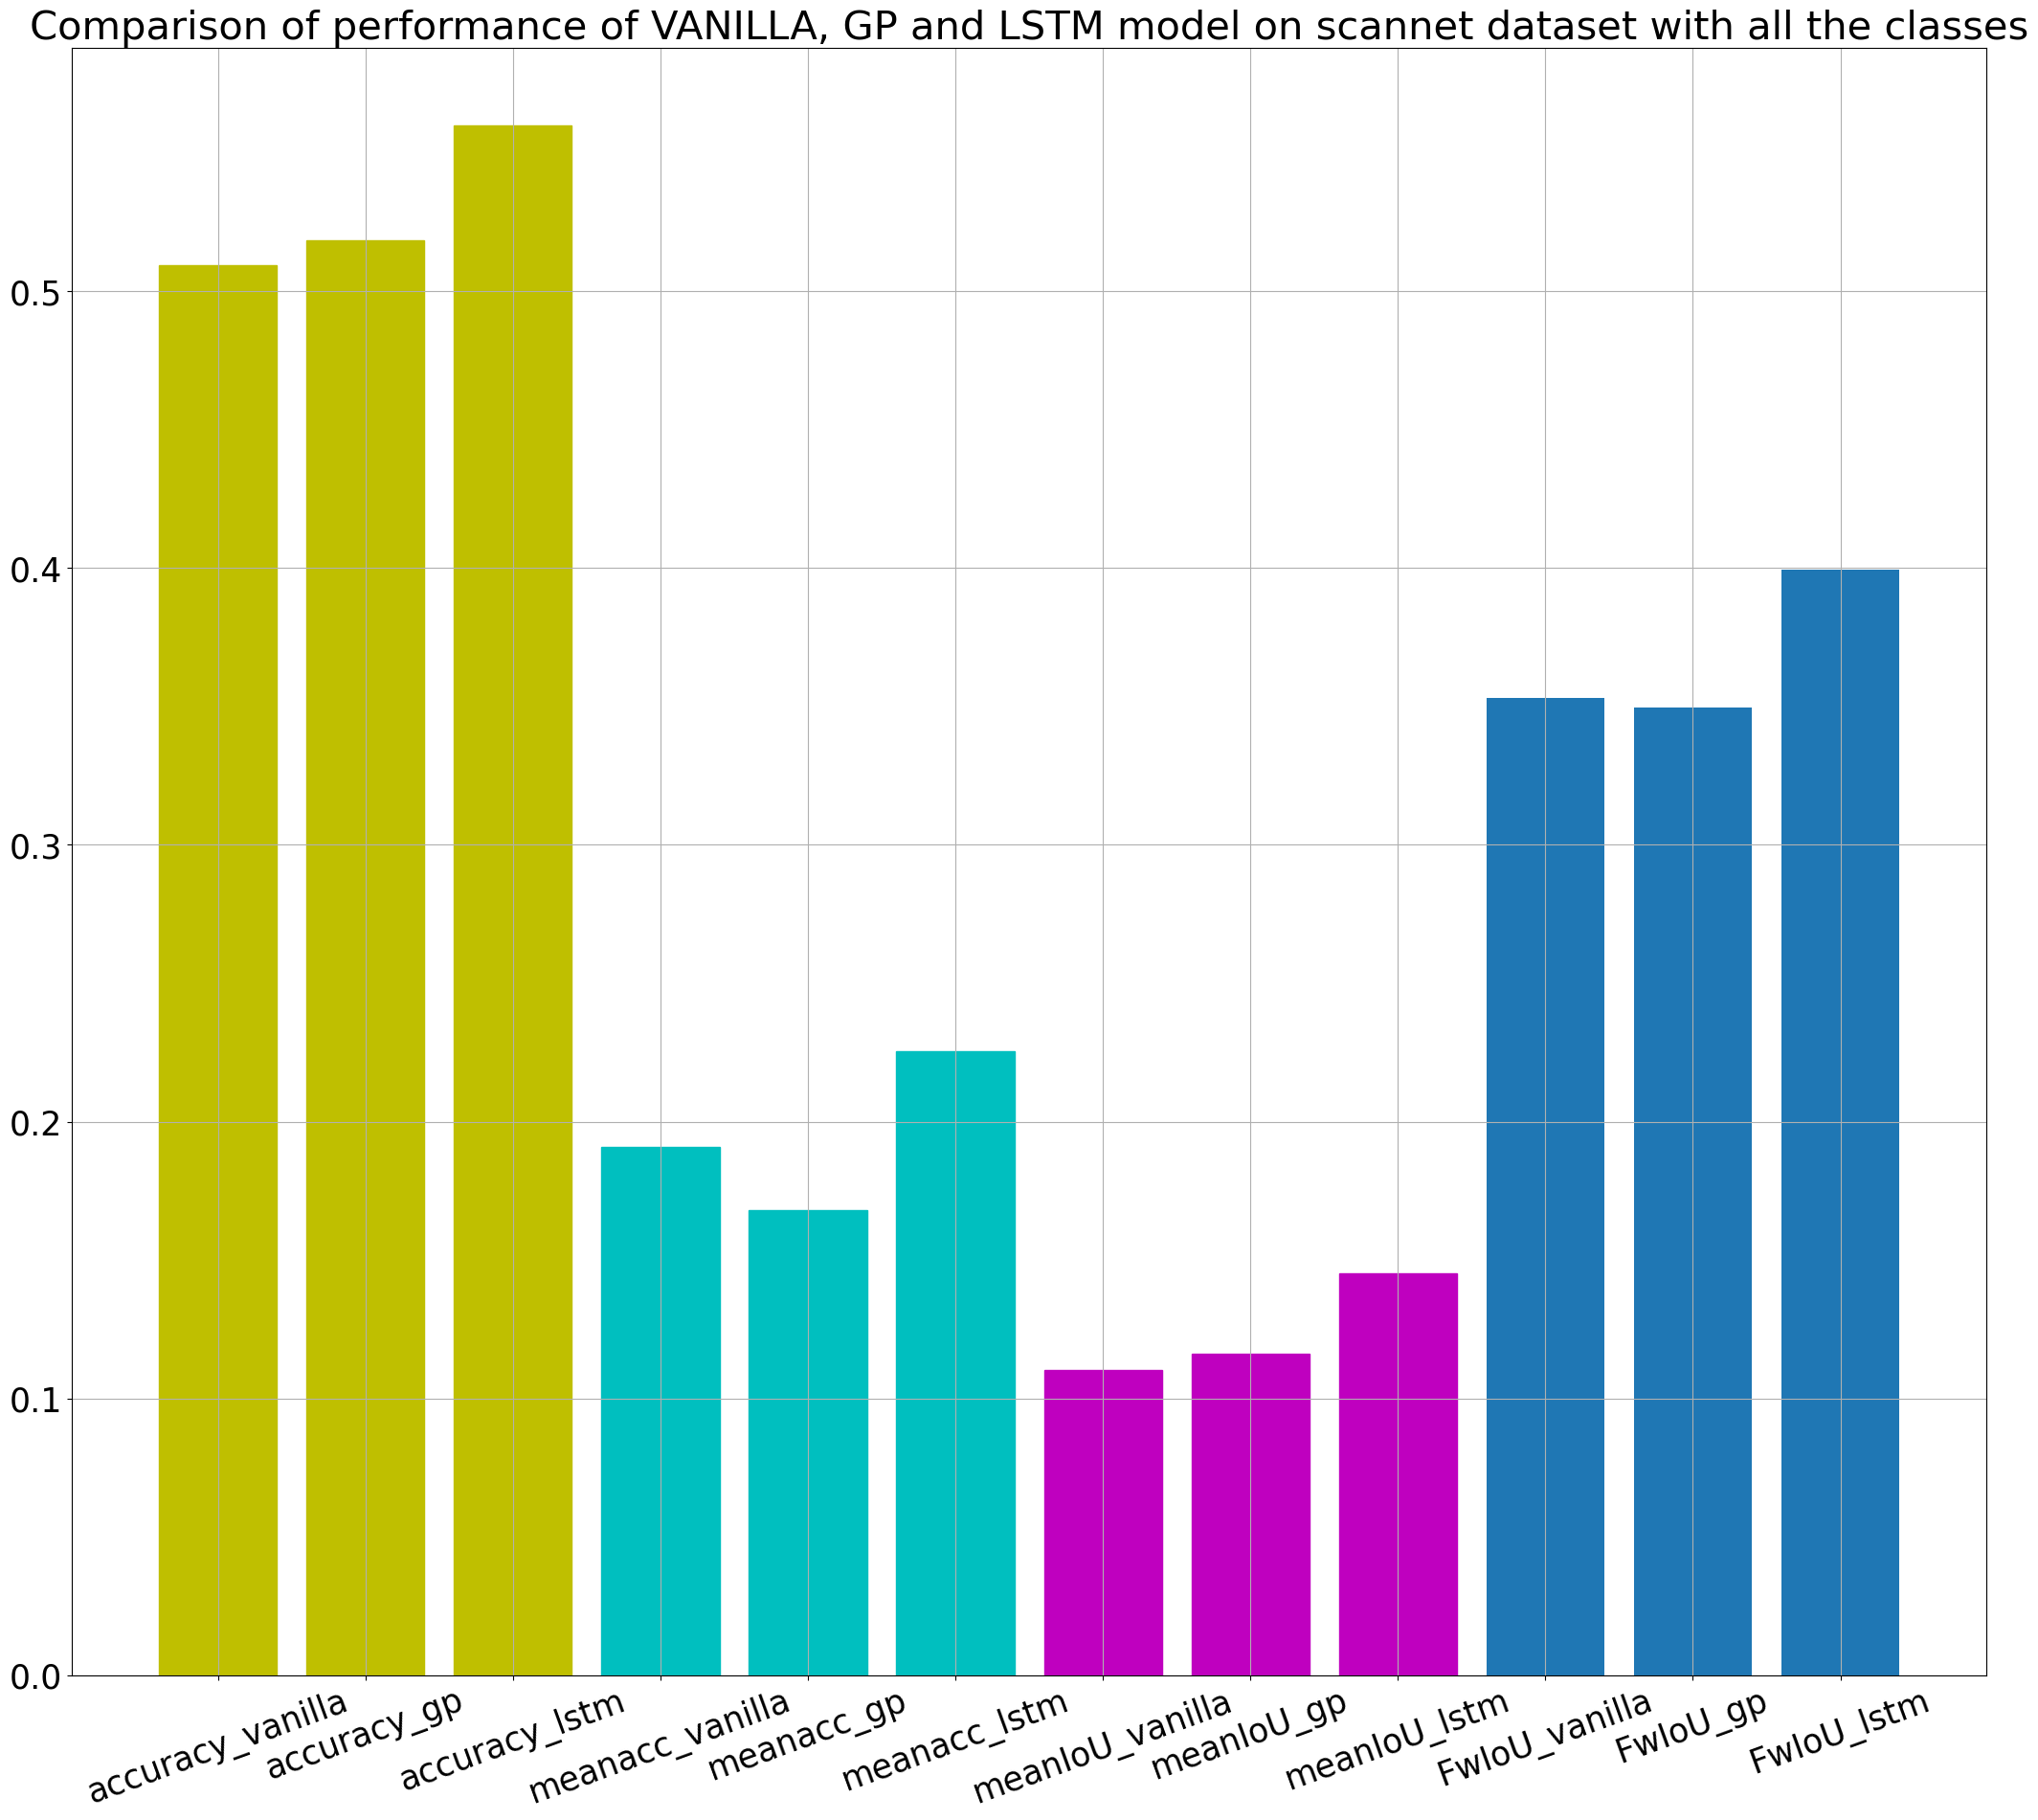
\includegraphics[width=12cm]{images/scannet_performance_all_classes.png}
		\caption{Comparison of VANILLA, GP and LSTM model performance based on metric}
		\label{fig:unet_model_metric_comparison_all_classes}
	\end{figure}
	
	\begin{figure}
		\centering
		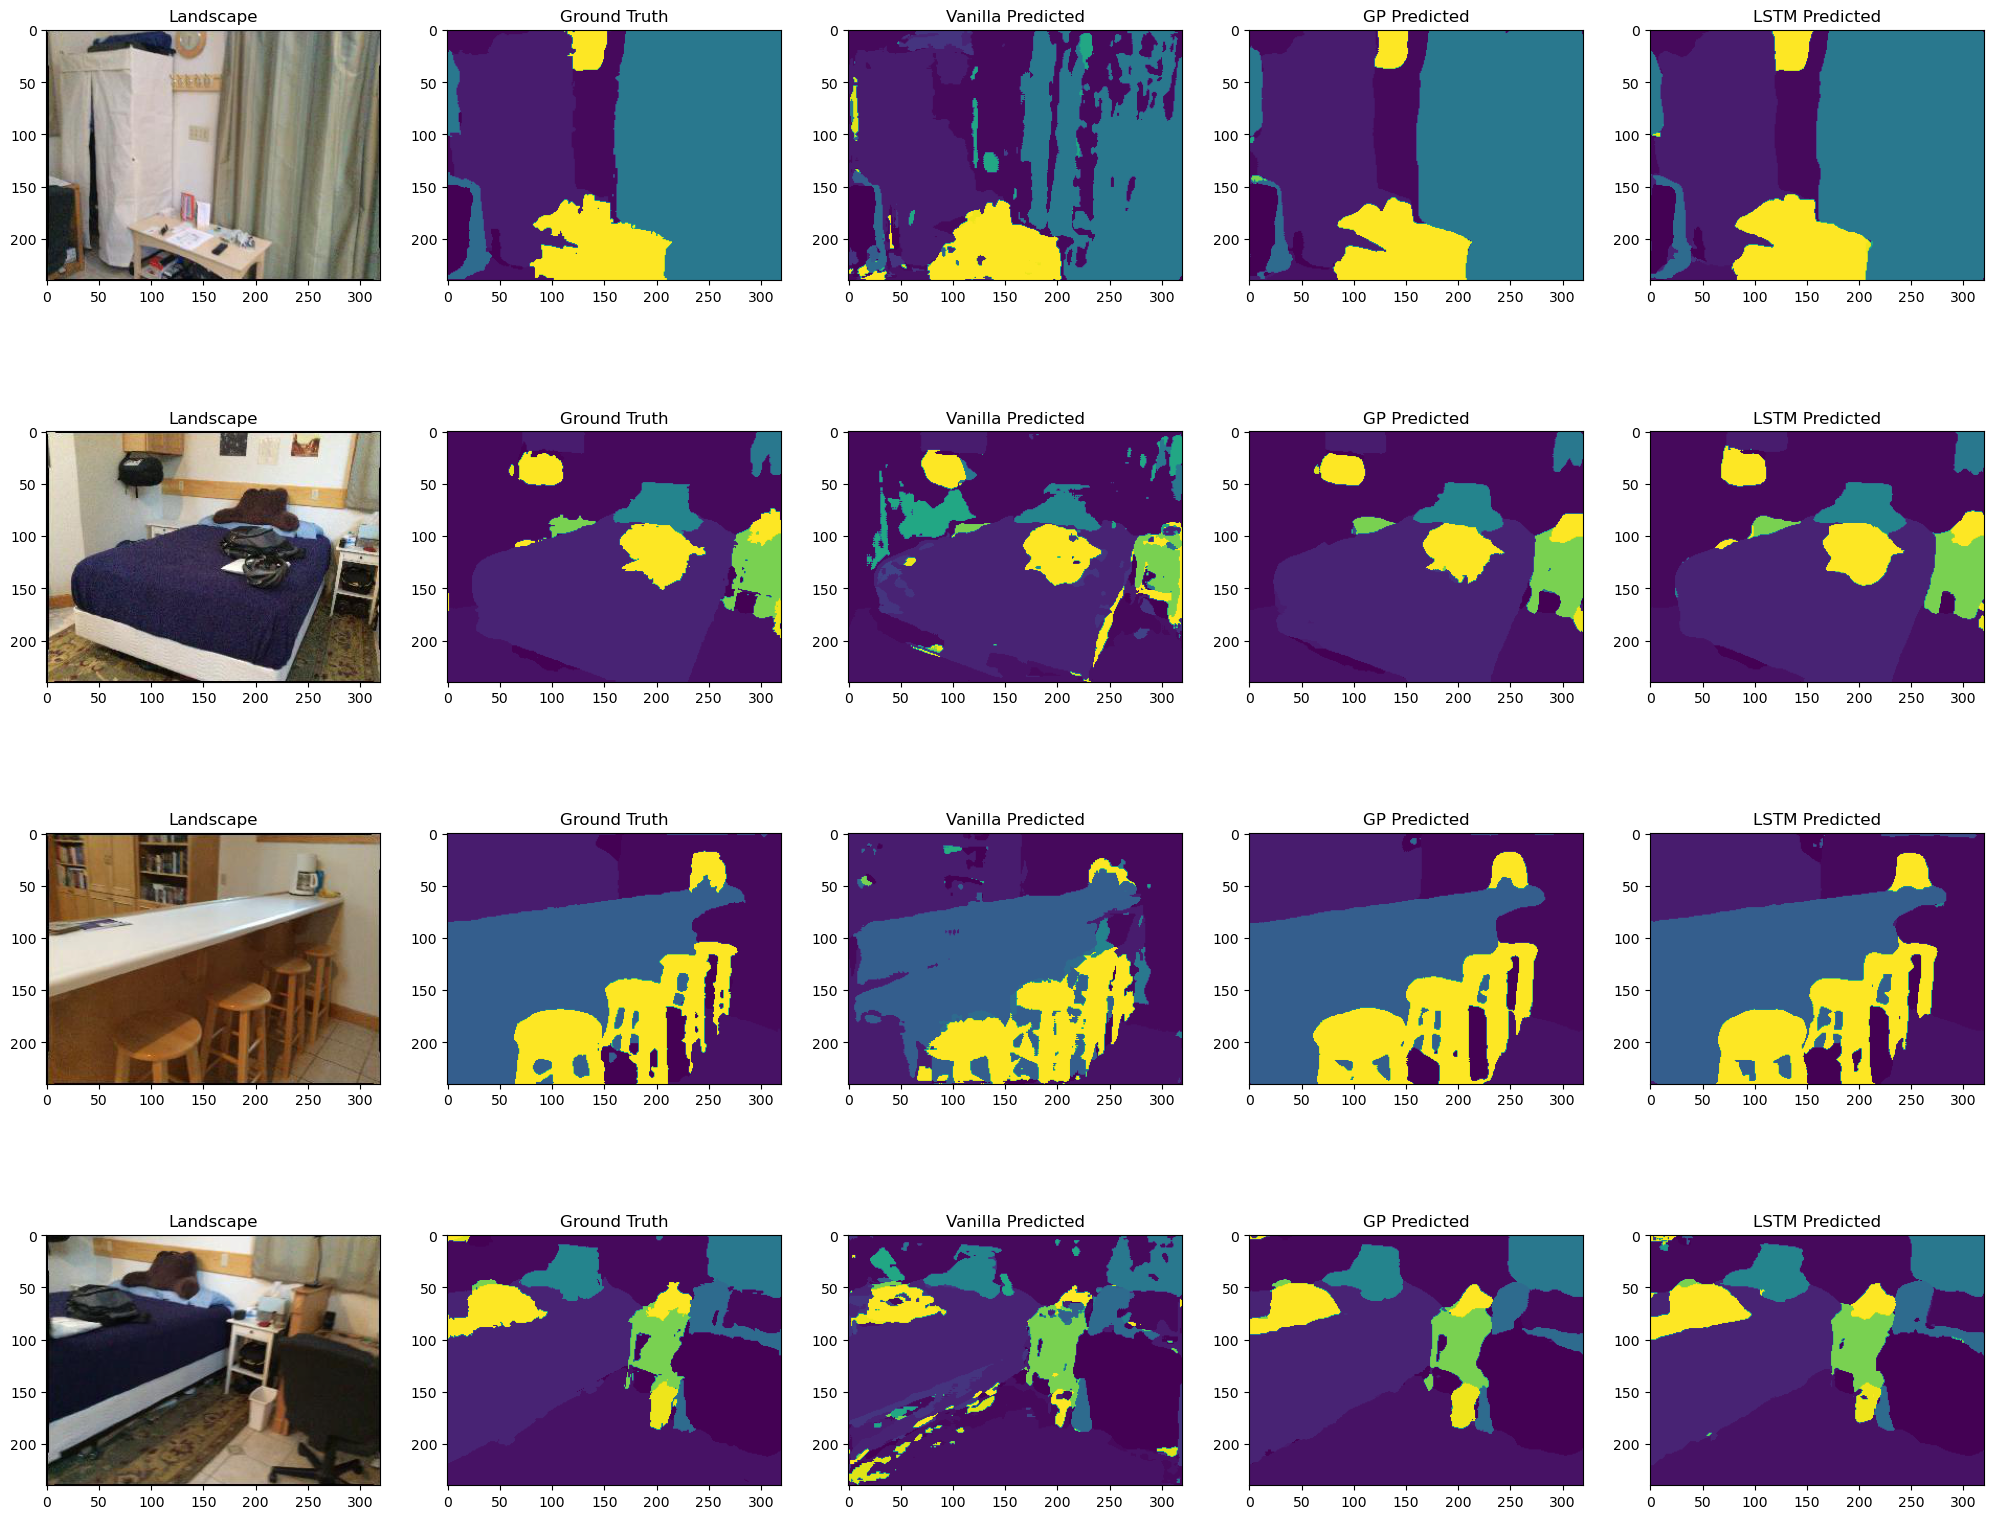
\includegraphics[width=16cm]{images/unet_scannet_all_classes.png}
		\caption{Comparison of VANILLA, GP and LSTM model performance}
		\label{fig:unet_model}
	\end{figure}

	\newpage
		
    \subsection{Experiment1.2: U-Net Vanilla, Temporally fused gp model and LSTM model considering two classes}
    %------------------------------------------------------------------------------------------------------
	In the second experiment on the scannet dataset all the classes are combined together except the wall class resulting in wall and other class. Table \ref{table:unet_two_classes} compares the results of vanilla, GP and LSTM model performance. In this case the pixel accuracy is similar in case of vanilla and the lstm model, however the accuracy dropped for the gp model. Similar observation can be made with the mean accuracy. However the meanIoU value is high for the lstm model at 0.28 and vanilla and gp produced a result of 0.14 and 0.23. The frequency weighted intersection over union is high for the lstm model followed by vanilla and gp model. Comparison of model output is presented in the Fig \ref{fig:output_vanilla}. In this case the wall and other categories in the test image are segmented reasonably well by the LSTM model. The metric bar comparison is shown in the Fig \ref{fig:unet_model_metric_comparison}. It is evident from the plot that the mean accuracy is good for the vanilla and gp and lstm performance is below the other models. However, the meanIoU and FWIoU is high for the lstm model.
	
	\begin{figure}[h]
		\centering
		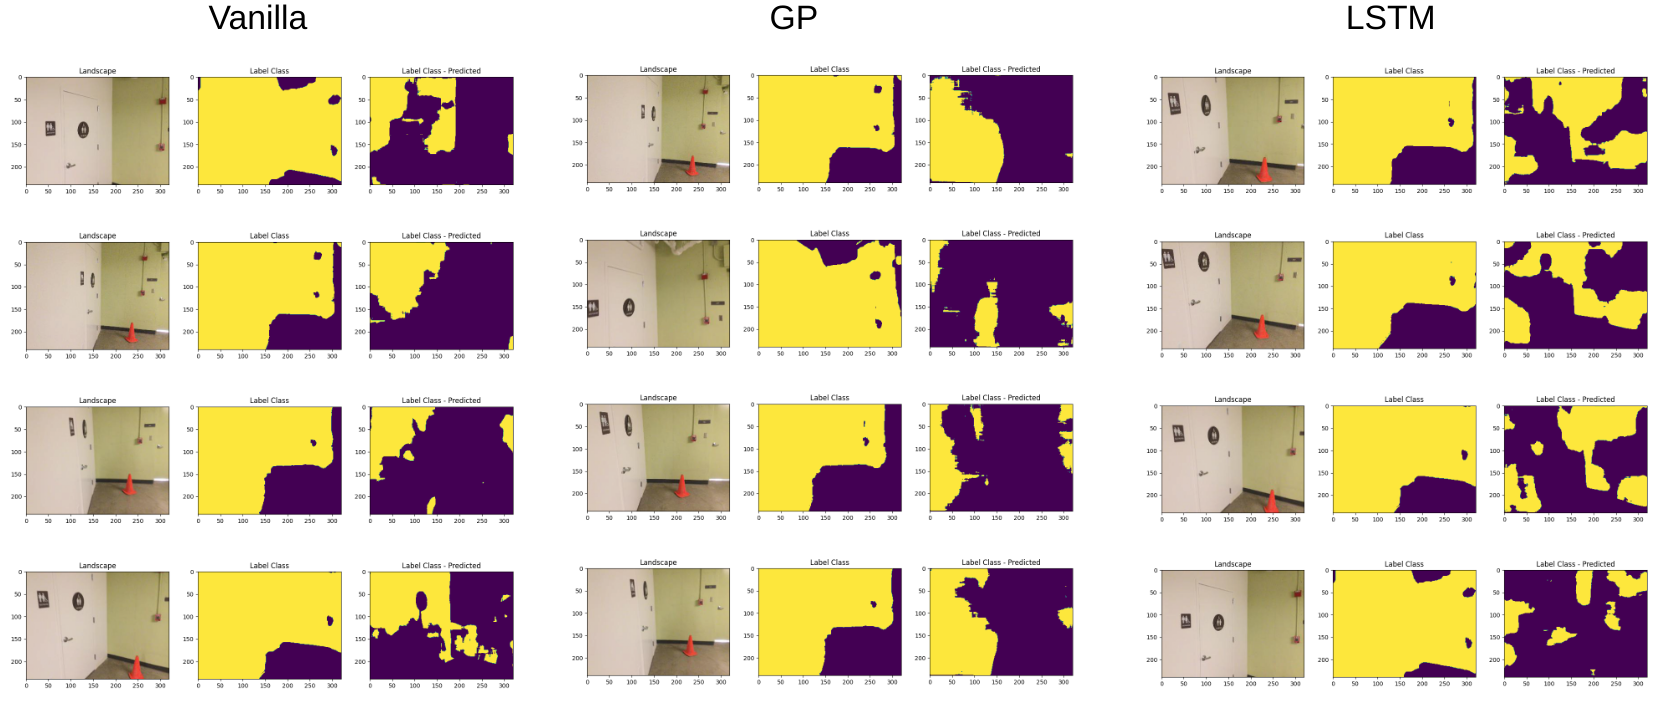
\includegraphics[width=16cm]{images/output_unet_two_classes.png}
		\caption{Plotting of raw input image, ground truth and predicted output for vanilla, gp and lstm model}
		\label{fig:output_vanilla}
	\end{figure}
	
	\begin{table}[h]
		\begin{center}
			\begin{tabular}{ | l | l | l | p{4cm} |}
				\hline
				
				\cellcolor{purple!30}Metric & \cellcolor{purple!30}Vanilla & \cellcolor{purple!30}GP & \cellcolor{purple!30}LSTM\\ \hline
				Pixel Accuracy & 0.4342 & 0.3764 & 0.8549\\ \hline
				Pixel Mean accuracy & 0.6232 & 0.5625 & 0.7837 \\ \hline
				meanIOU & 0.145 & 0.2318 & 0.6593 \\ \hline
				IoU & [0.2737, 0.2809] & [0.2377, 0.2259] & [0.8280, 0.4903] \\ \hline
				FwIoU & 0.2793 & 0.2284 & 0.7643 \\ \hline
				\hline
			\end{tabular}
			\caption{Performance of Vanilla model with respect to different metric and two classes}
			\label{table:unet_two_classes}
		\end{center}
	\end{table}
	
	
	\begin{figure}
		\centering
		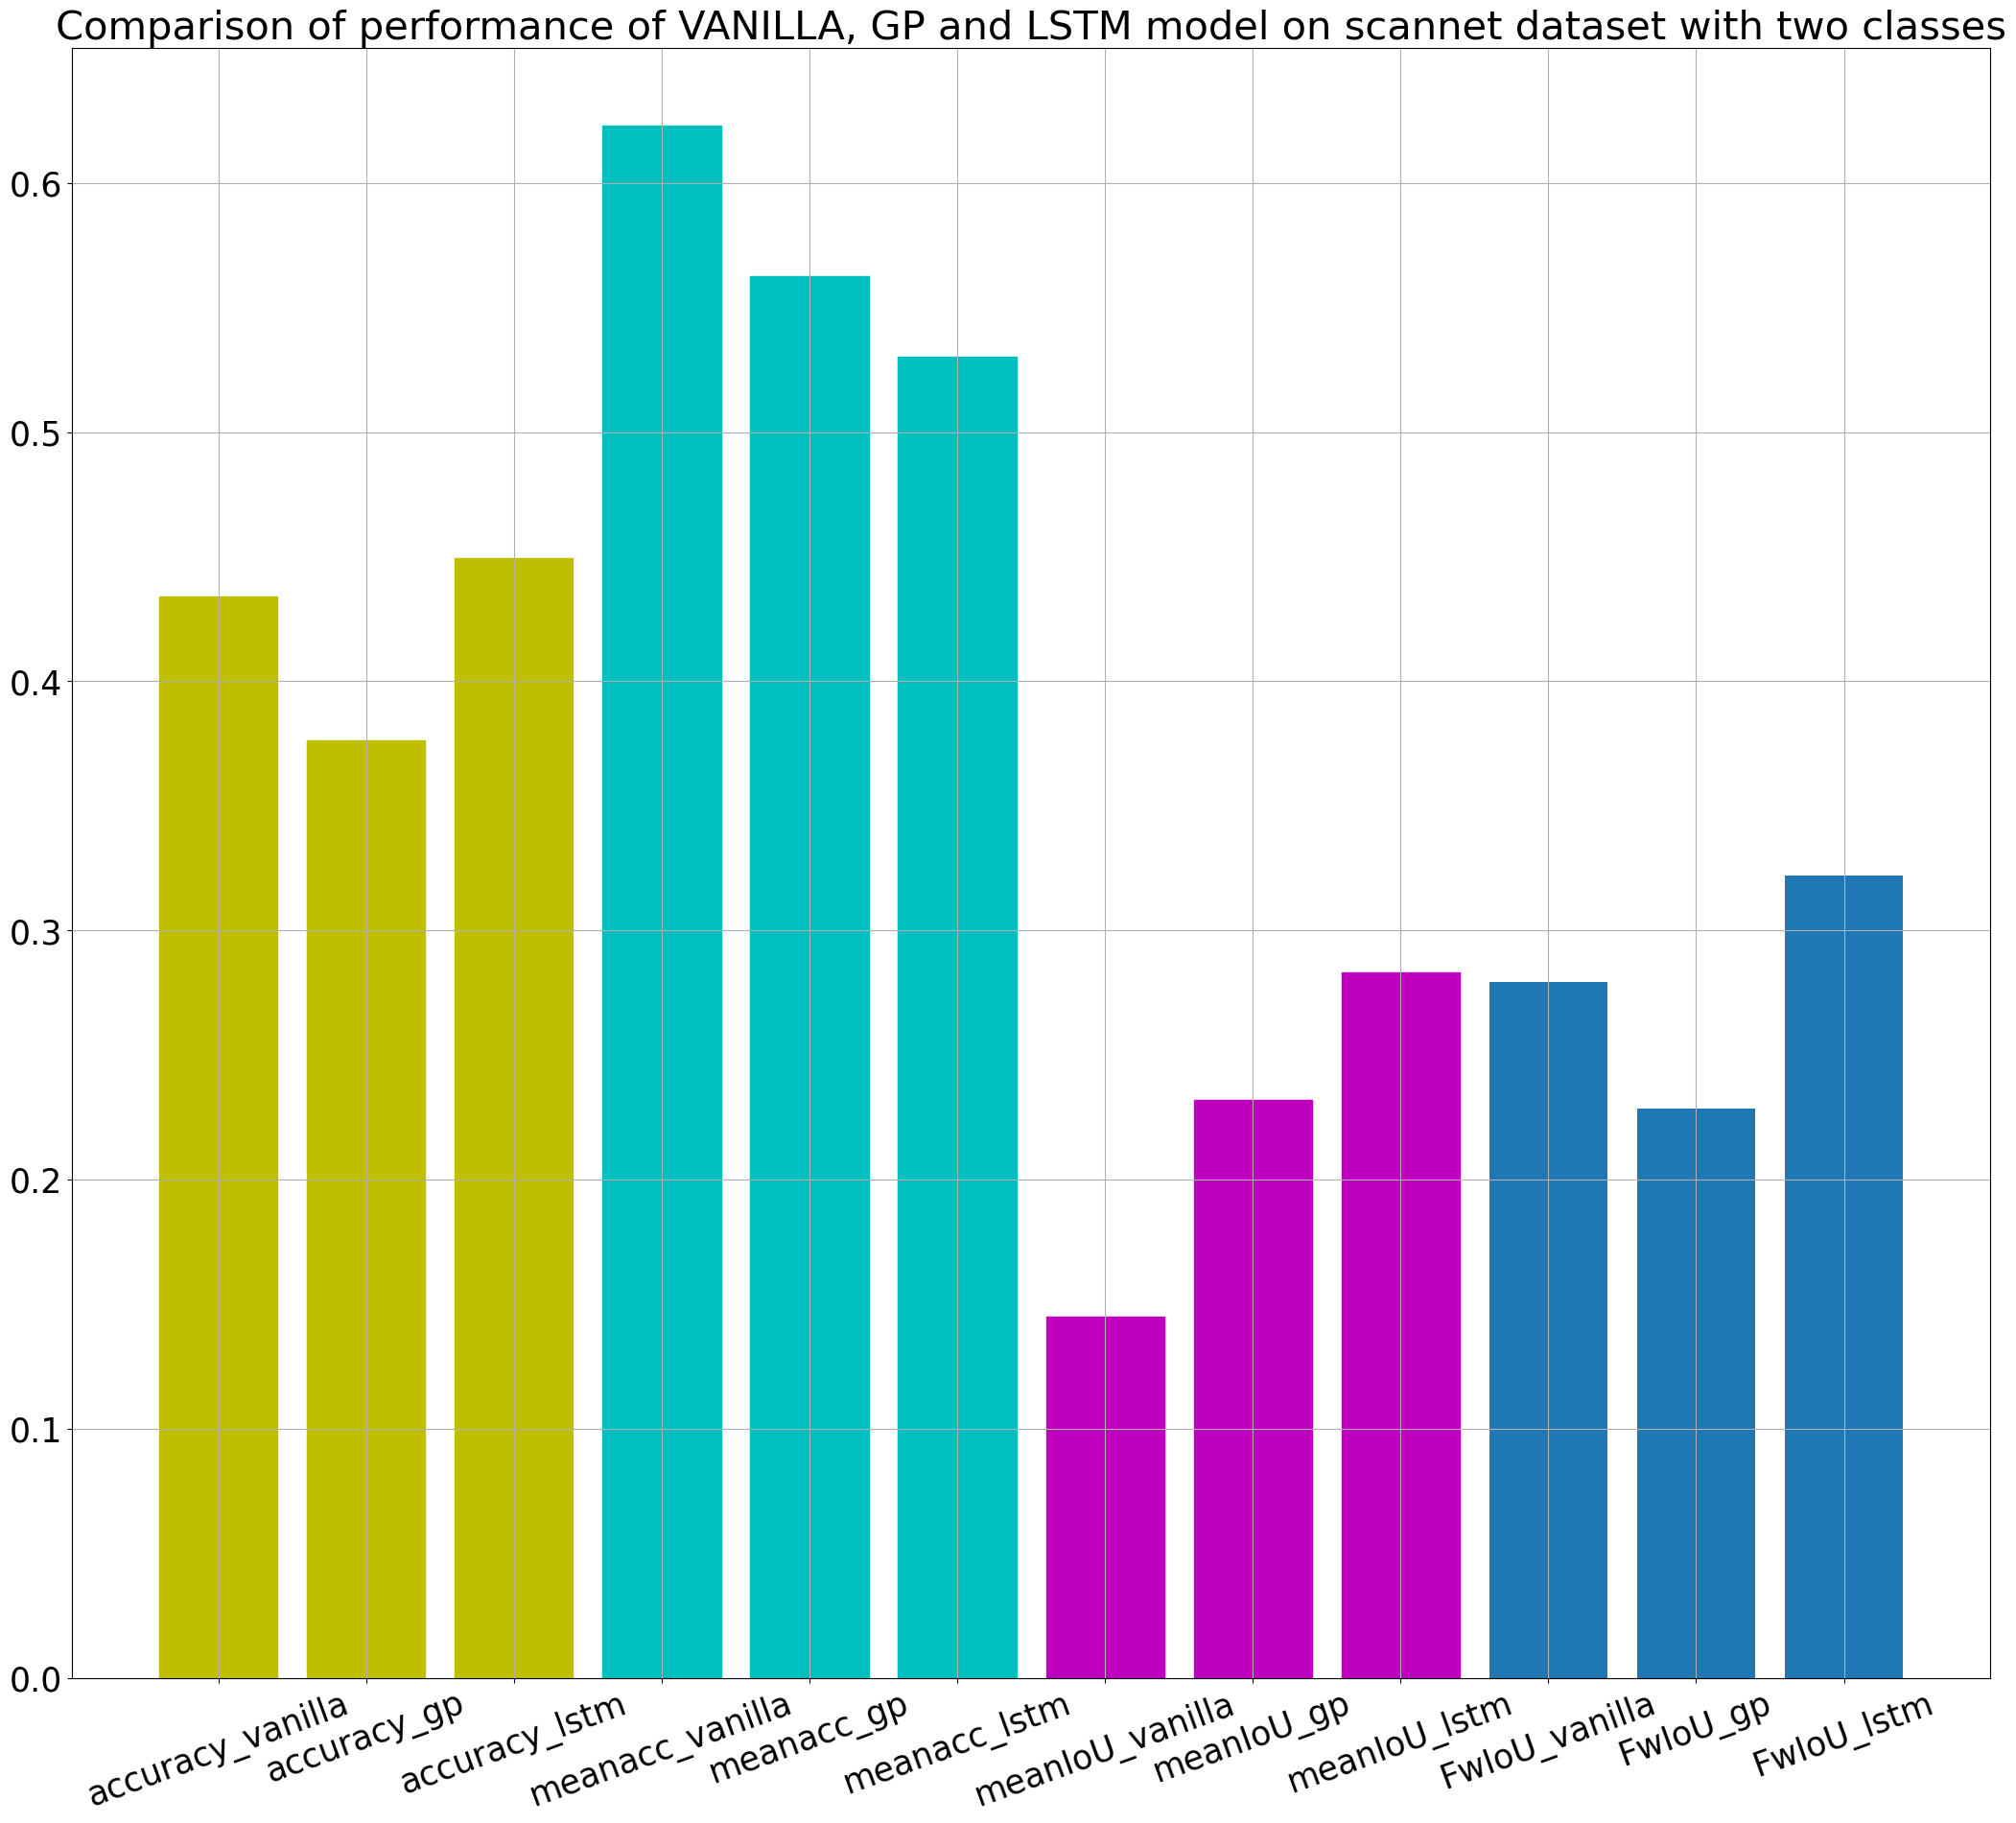
\includegraphics[width=12cm]{images/scannet_performance_two_classes.png}
		\caption{Comparison of VANILLA, GP and LSTM model performance based on metric for scannet two classes}
		\label{fig:unet_model_metric_comparison}
	\end{figure}

    %------------------------------------------------------------------------------------------------------
    \subsection{Experiment1.3: U-Net Vanilla, temporally fused gp and lstm model considering three classes}
	
	In this experiment wall, furniture and other+combined classes are considered due to high pixel distribution, resulting in three unique classes. There is a huge jump in the pixel accuracy for the lstm and gp model in comparison to vanilla model. The mean pixel accuracy is high at 0.55 in comparison to vanilla model performance at 0.31. A increase of 24\%. The meanIoU value also stand high at 0.40 for lstm model in comparison to 0.18 for vanilla model, a difference of 22\%. The FwIoU value increased by 25\% for the lstm model. The effect of temporal fusion can be clearly seen with these metrics. Temporal fusion improved the performance by a huge margin. The gp model also performed well in comparison with vanilla and lstm. In this experiment the pixel classes are well balanced in comparison with the two class approach, where the difference is high. The comparison of results are presented in the table Table \ref{table:unet_scannet_three_classes}. Temporal fusion in action can be seen in Fig \ref{fig:performance_metric_three_classes_scannet}. The comparison of model performance with a bar plot is depicted in Fig \ref{fig:performance_metric_three_classes_unet}
	
	\begin{figure}
		\centering
		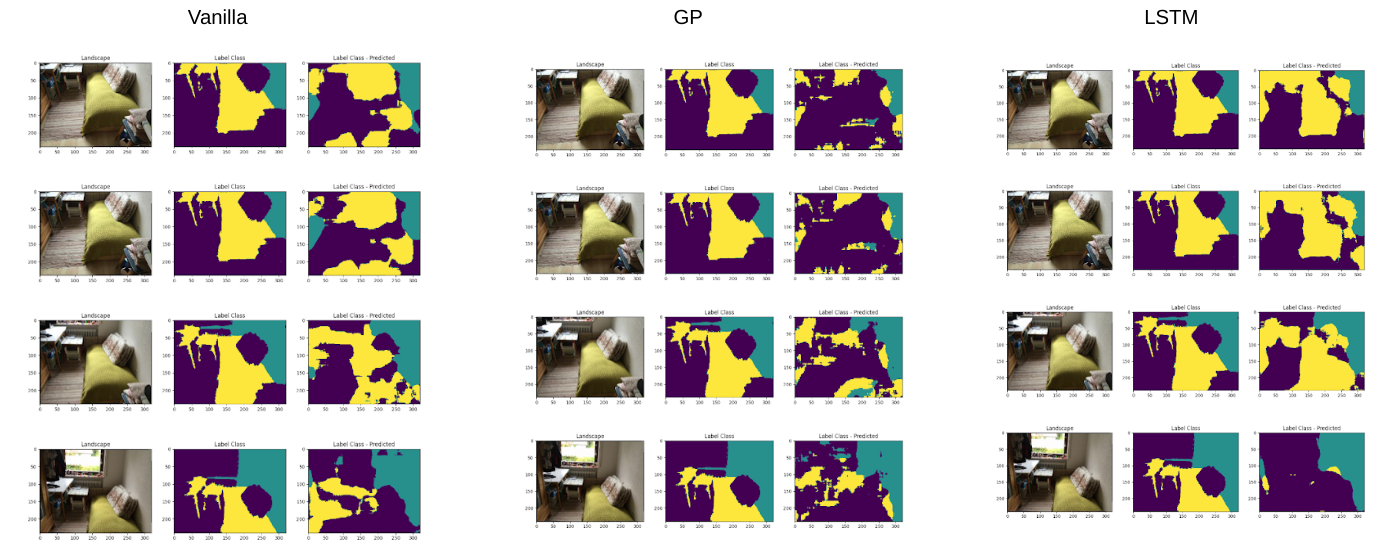
\includegraphics[width=16cm]{images/unet_scannet_three_classes.png}
		\caption{Plotting of raw input image, ground truth and predicted output for vanilla, gp and lstm model}
		\label{fig:performance_metric_three_classes_scannet}
	\end{figure}

	\begin{table}[h]
		\begin{center}
			\begin{tabular}{ | l | l | l | p{4cm} |}
				\hline
				
				\cellcolor{purple!30}Metric & \cellcolor{purple!30}Vanilla & \cellcolor{purple!30}GP & \cellcolor{purple!30}LSTM\\ \hline
				Pixel Accuracy & 0.3289 & 0.5731 & 0.6266 \\ \hline
				Pixel Mean accuracy & 0.3135 & 0.4779 & 0.6920 \\ \hline
				meanIOU & 0.1820 & 0.3356 & 0.4870 \\ \hline
				IoU & [0.2732, 0.1686, 0.1042] & [0.5178, 0.3066, 0.1823] & [0.6810, 0.4661, 0.2998] \\ \hline
				FwIoU & 0.2160 & 0.4033 & 0.6245 \\ \hline
				\hline
			\end{tabular}
			\caption{Performance of Vanilla model with respect to different metric and two classes}
			\label{table:unet_scannet_three_classes}
		\end{center}
	\end{table}	
	
	\begin{figure}
		\centering
		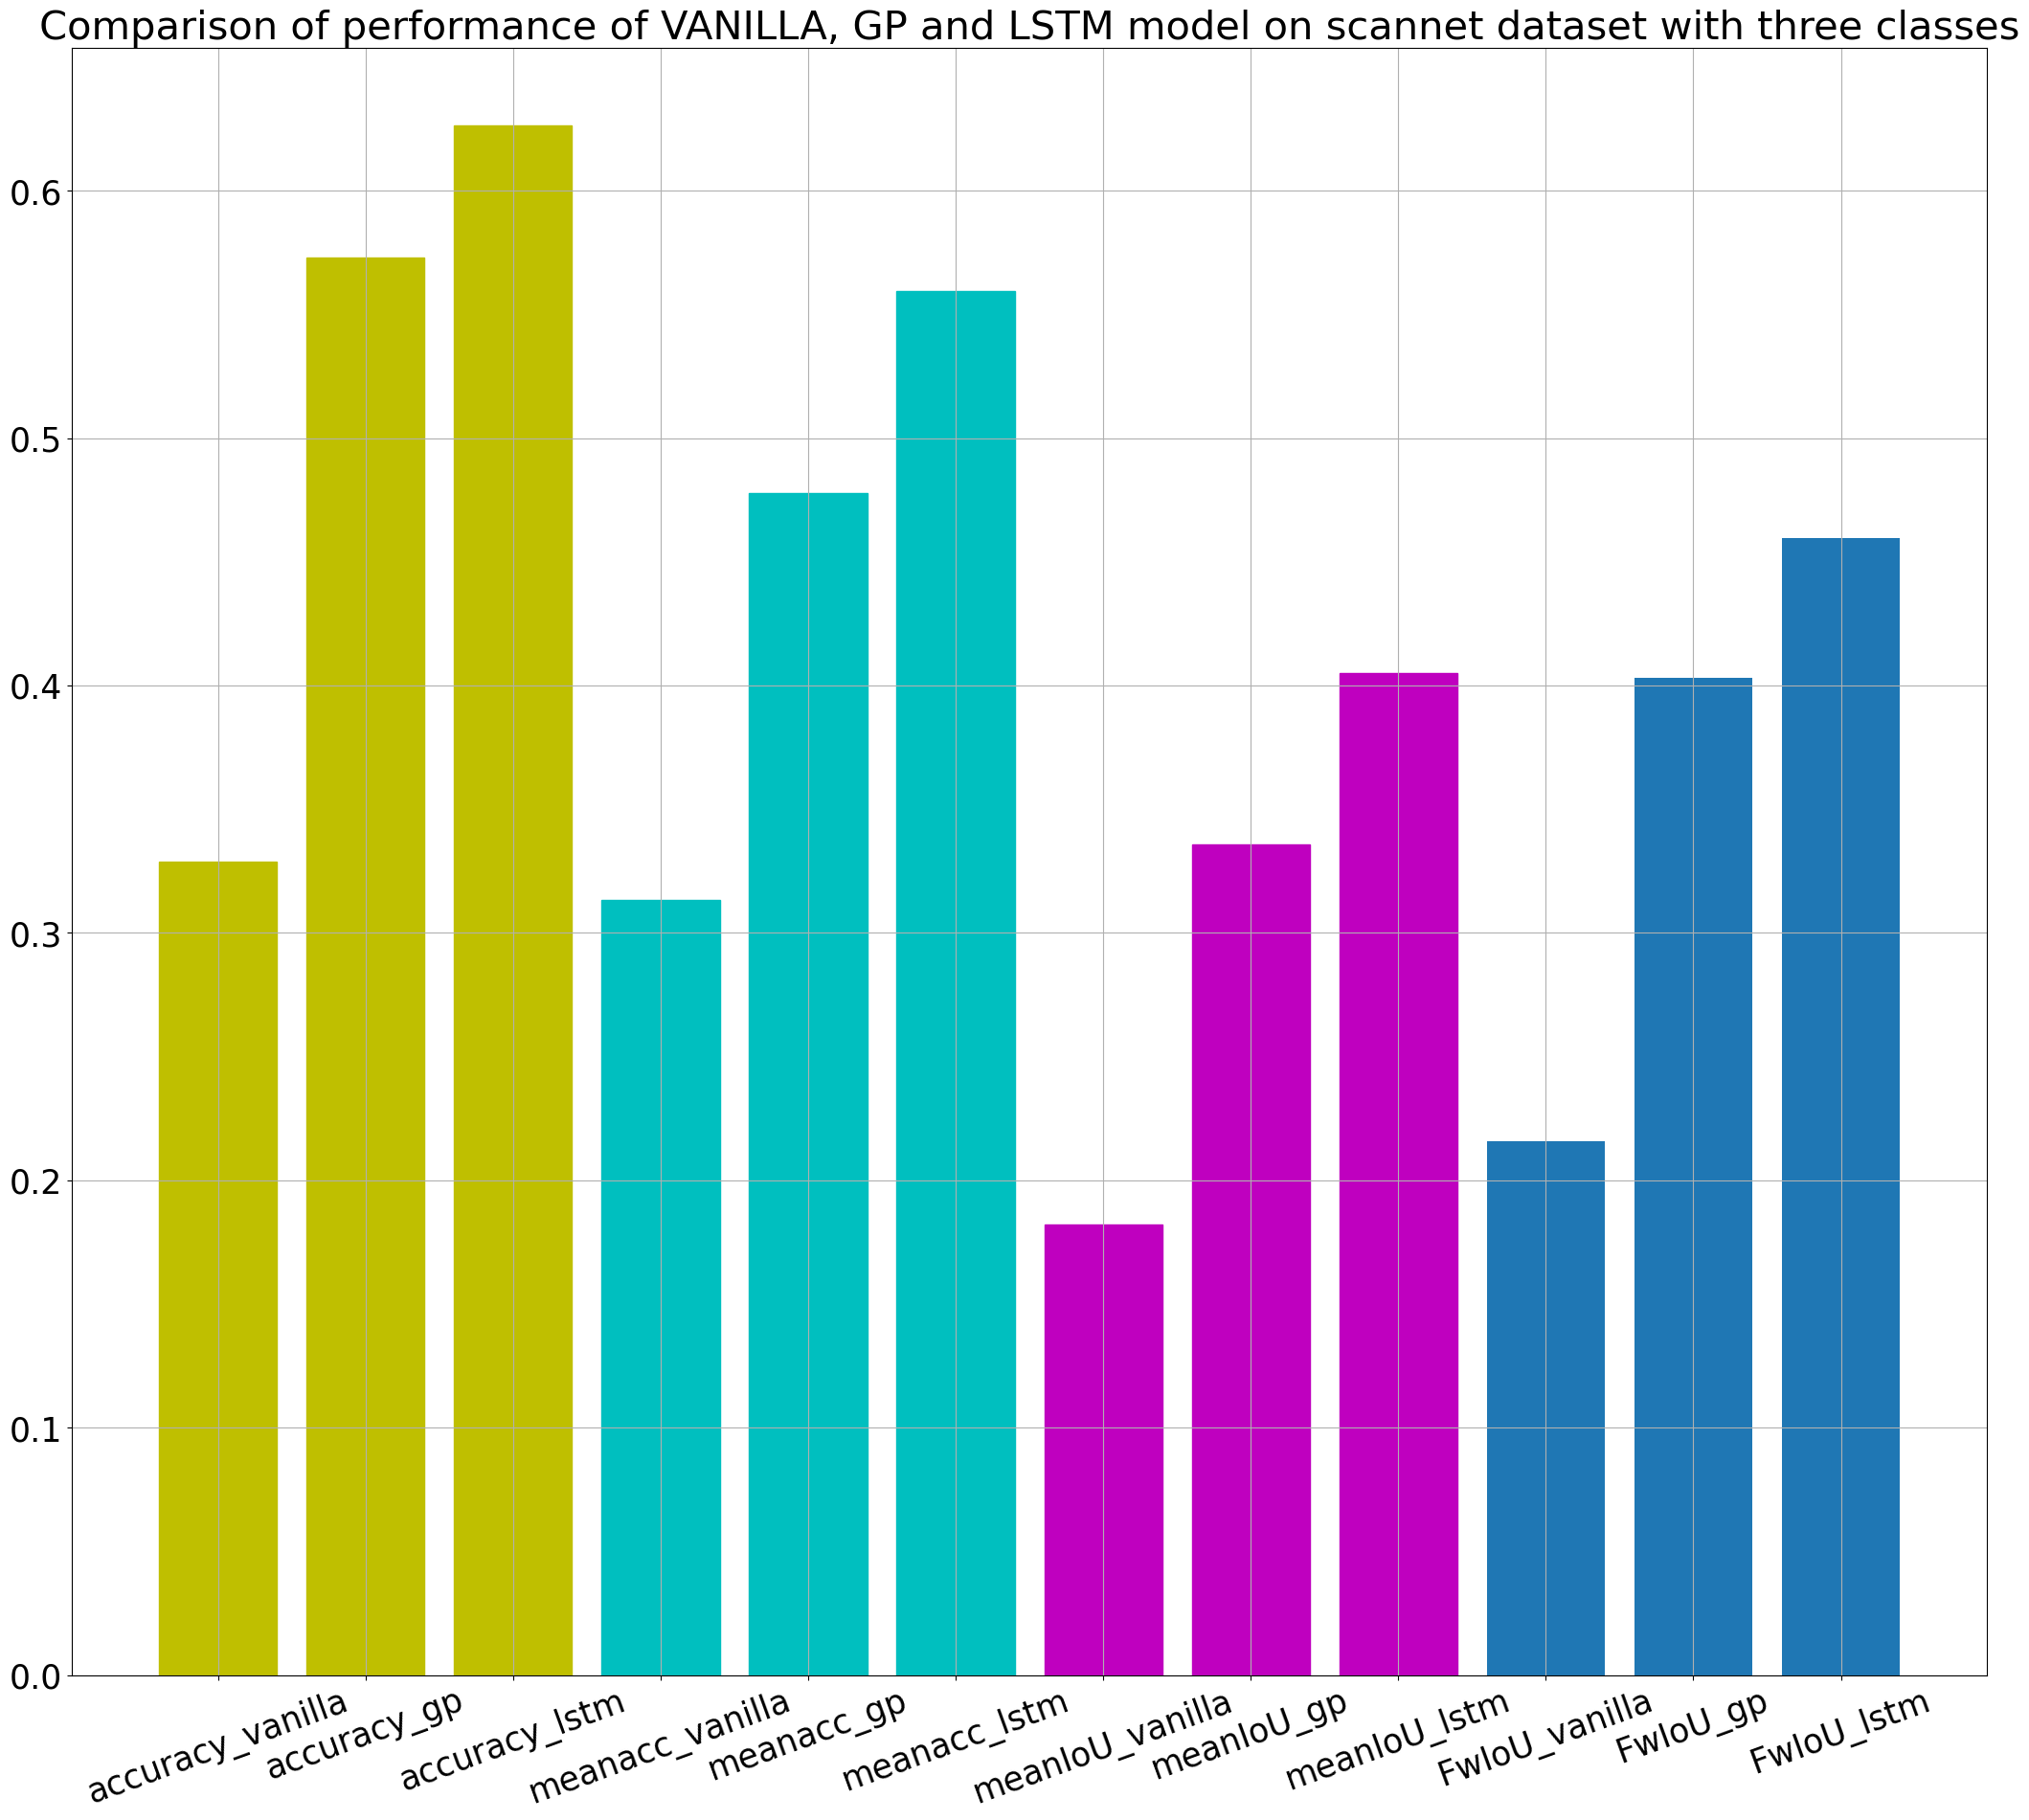
\includegraphics[width=12cm]{images/scannet_performance_three_classes.png}
		\caption{Plotting of raw input image, ground truth and predicted output for vanilla, gp and lstm model}
		\label{fig:performance_metric_three_classes_unet}
	\end{figure}

	\newpage
	\newpage
	%\subsection{Discussion on comparison of results for Vanilla, GP and LSTM models performance}
	
	\section{Experiment 2.1: Experiment with vkitti dataset with clone and sunset as the testing data}
	
	Similar to the experiments conducted on the scannet dataset, experiments were conducted on the vkitti dataset. Vkitti is a dataset containing a virtual car moving in a city scape and recorded with different configuration. There are totally 15 classes in the entire dataset. The results were tabulated in the Table \ref{table:unet_vkitti_two_classes}. There are totally 10 categories in the entire dataset. In this experiment clone and sunset are taken as the testing data and trained on the remaining 8 classes. The result of the experiments were tabulated in the Table \ref{table:unet_vkitti_two_classes}. The Vanilla, GP and LSTM model performance are compared in the table. A small improvement in the performance can be observed due to the similarity between the all the different categories. All the categories are similar, only the environment changes. In this experiment GP performed well in comparison to the vanilla and LSTM model. The accuracy of the model is high 0.98. Temporal fusion can be observed with mean pixel accuracy, FwIoU and meanIoU metric with improvement in result. The model is evaluated with the testing data and the results are calculated for every batch and plotted as the box plot in the Fig \ref{fig:performance_metric_vkitti_two_class_box_plot}. For all of the metric the GP produced better result in comparison other models. IoU for the traffic light, pole was low with respect to the other classes. The performance of vanilla and the LSTM model is similar. Four test images were taken and run through vanilla, GP and LSTM model and the ground truth and the predictions are compared side by side. Vanilla and GP model perfectly segment the truck, however the LSTM model not properly segment the truck. However, car, pole, road, sky categories are perfectly categorized by these models. The side by side comparison is presented in the Figure \ref{fig:vkitti_unet_two}. 
	
	\begin{figure}[h]
		\centering
		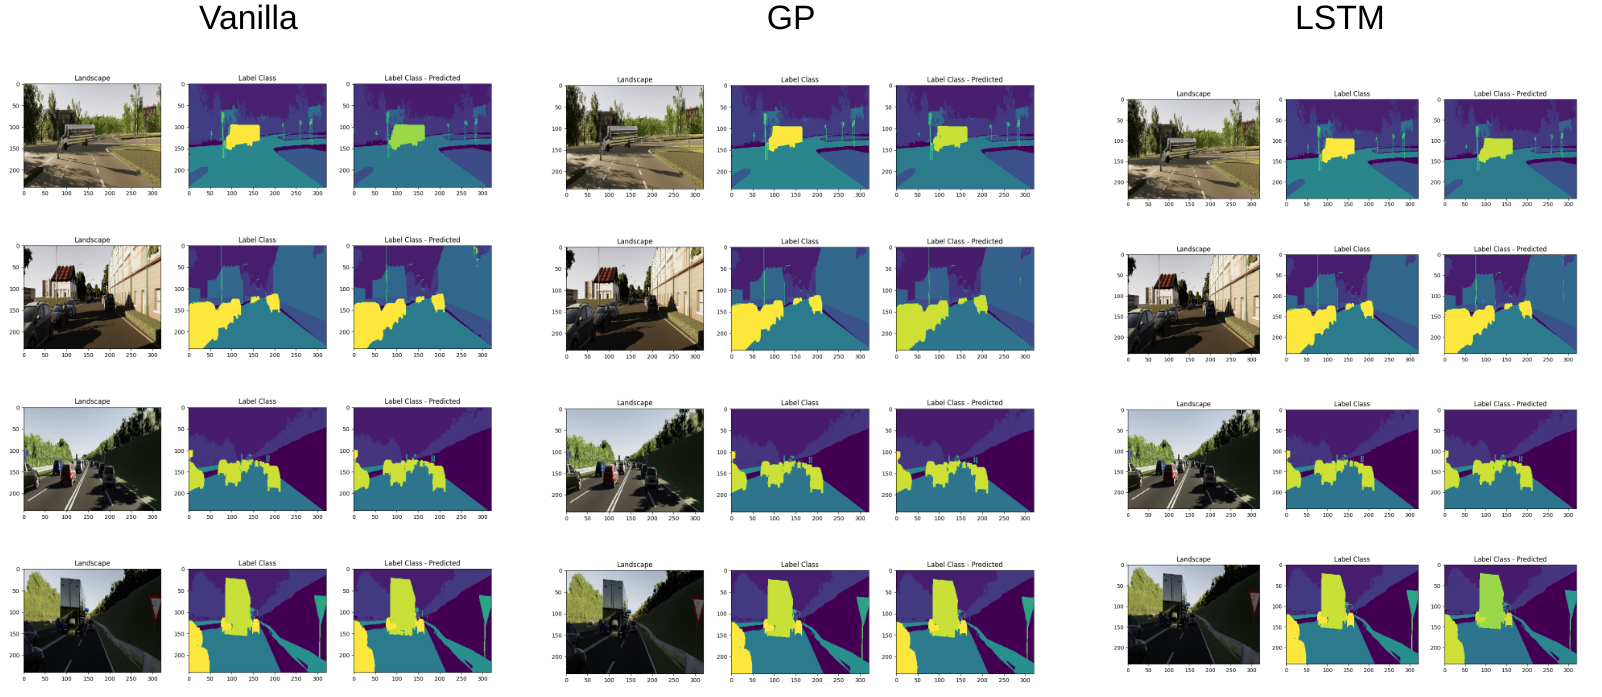
\includegraphics[width=17cm]{images/unet_vkitti_two.png}
		\caption{Plotting of raw input image, ground truth and predicted output for vanilla, gp and lstm}
		\label{fig:vkitti_unet_two}
	\end{figure}

	\begin{table}
		\begin{center}
			\begin{tabular}{ | l | p{4cm} | p{4cm} | p{4cm} |}
				\hline
				
				\cellcolor{purple!30}Metric & \cellcolor{purple!30}Vanilla & \cellcolor{purple!30}GP & \cellcolor{purple!30}LSTM\\ \hline
				
				Pixel Accuracy & 0.9835 & 0.9857 & 0.9843 \\ \hline
				Pixel Mean accuracy & 0.9572 & 0.9637 & 0.9596 \\ \hline
				meanIOU & 0.9241 & 0.9364 & 0.9279 \\ \hline
				IoU & [0.9714, 0.9731, 0.966, 0.9377, 0.9296, 0.9894, 0.9663, 0.9265, 0.8165, 0.7835, 0.8359, 0.9474, 0.9633, 0.9299] & 
				[0.9752, 0.9741, 0.9685, 0.955, 0.9393, 0.9918, 0.9714, 0.9413, 0.822, 0.8195, 0.8686, 0.9618, 0.9705, 0.9497] 
				& [ 0.9732, 0.9736, 0.9664, 0.9482, 0.9289, 0.9906, 0.9693, 0.9313, 0.8135, 0.7837, 0.8492, 0.9595, 0.9653, 0.9373]
				\\ \hline
				FwIoU & 0.9679 & 0.9721 & 0.9694 \\ \hline
				\hline
			\end{tabular}
			\caption{Performance of Vanilla model with respect to different metric and two classes}
			\label{table:unet_vkitti_two_classes}
		\end{center}
	\end{table}
	
	\begin{figure}
		\centering
		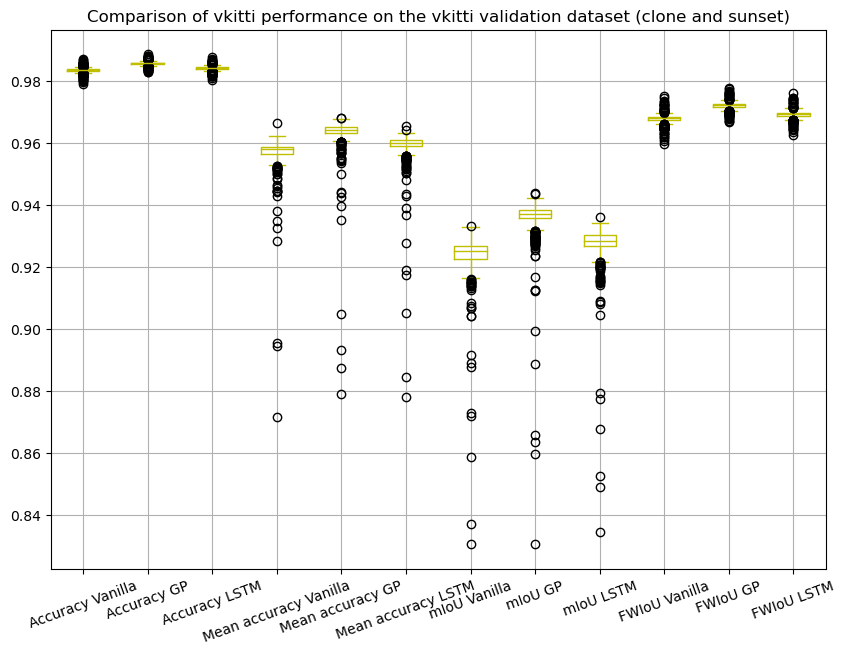
\includegraphics[width=12cm]{images/vkitti_validation_data_two_class_box_plot.png}
		\caption{Plotting of raw input image, ground truth and predicted output for vanilla, gp and lstm}
		\label{fig:performance_metric_vkitti_two_class_box_plot}
	\end{figure}
	
	\begin{figure}
		\centering
		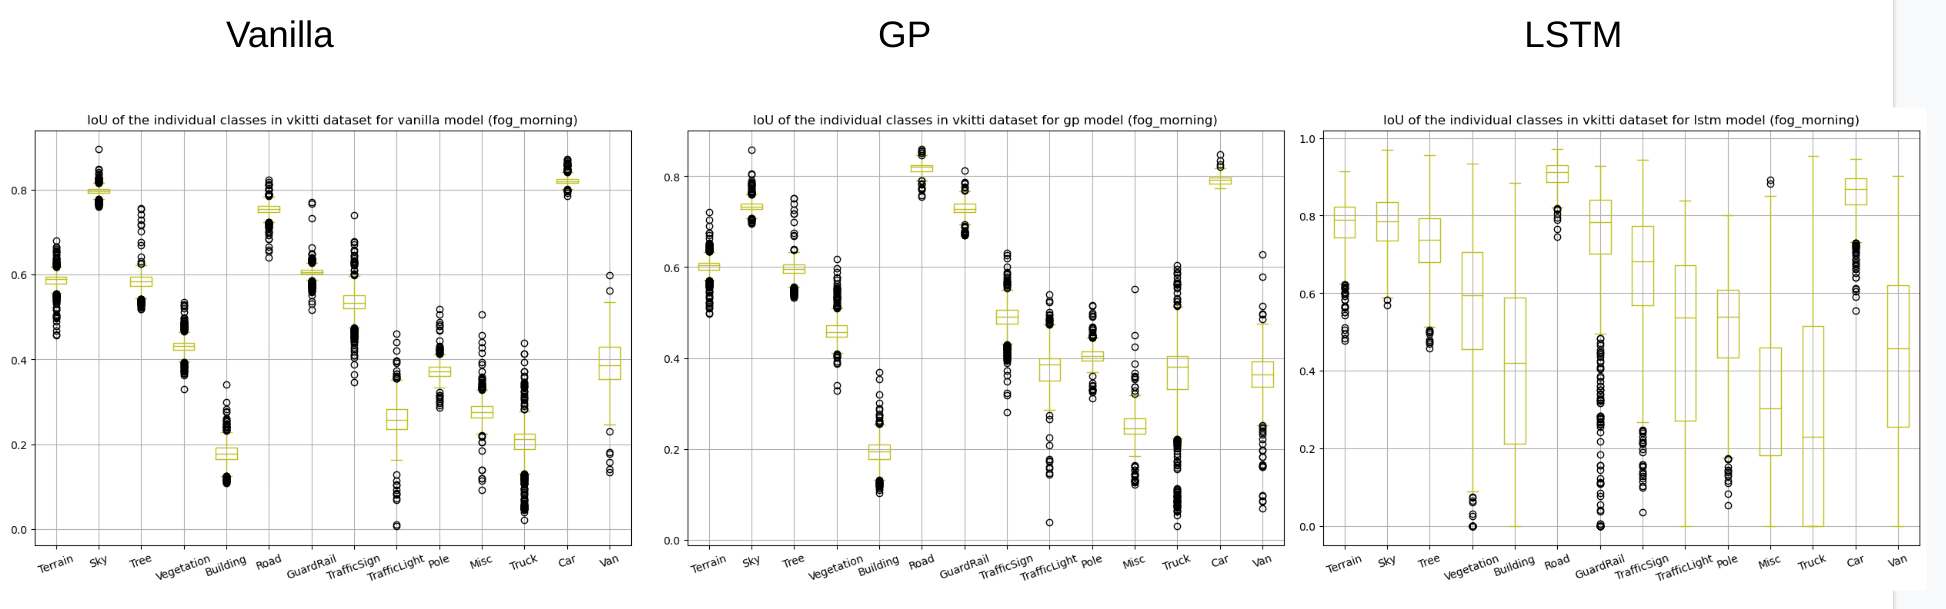
\includegraphics[width=19cm]{images/IoU_two.png}
		\caption{Plotting of raw input image, ground truth and predicted output for vanilla, gp and lstm}
		\label{fig:performance_metric_three_classes}
	\end{figure}

	\section{Experiment 2.2: Experiment with vkitti dataset with clone, sunset, rain, 15-deg-right, and 30-deg-left as the testing data}
	
	In the second type of experiment on vkitti data, five('clone/', 'sunset/', 'rain/', '15-deg-right/',
	'30-deg-left/') categories out of 10 categories are taken for testing. The model is trained on five (15-deg-left/','fog/', 'overcast/', 'morning/', '30-deg-right/') categories. The result of the experiments are tabulated in the Table \ref{table:Vanilla_conti_seq}. It is a side by side comparison of the model performance based on different metric. The performance improvement can be observed with the menIoU metric. The meanIoU improved by 1\% and 3\% for gp and lstm with respect to the vanilla model. Similar characteristics can be observed with the mean pixel accuracy. However, the pixel accuracy remained constant for the all the three model. The side by comparison of the raw rgb image, ground truth and predicted segmentation map is shown in the Fig \ref{fig:unet_side_by_side_five_classes}. 
	
	\begin{figure}
		\centering
		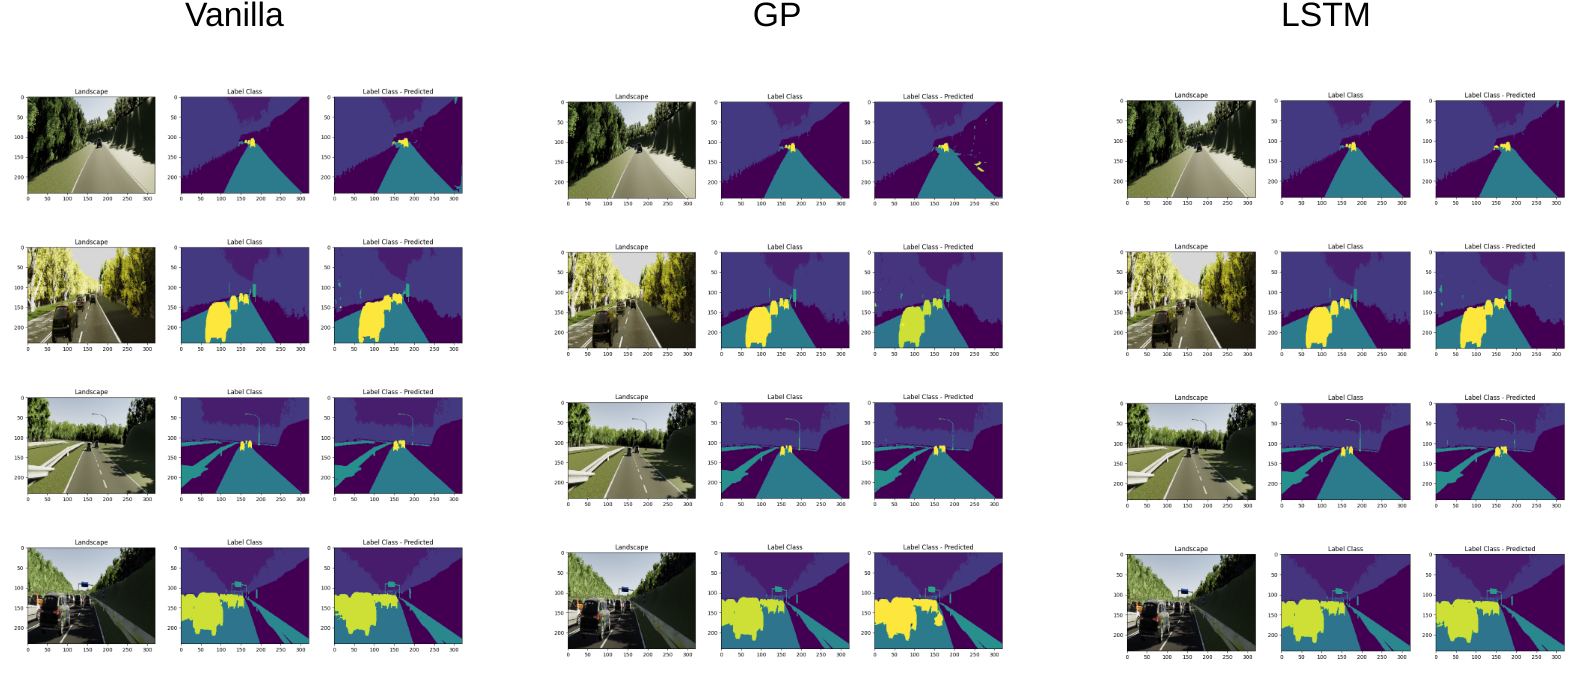
\includegraphics[width=17cm]{images/unet_vkitti_five.png}
		\caption{Plotting of raw input image, ground truth and predicted output for vanilla, gp and lstm}
		\label{fig:unet_side_by_side_five_classes}
	\end{figure}

	\begin{table}
		\begin{center}
			\begin{tabular}{ | l | p{4cm} | p{4cm} | p{4cm} |}
				\hline
				
				\cellcolor{purple!30}Metric & \cellcolor{purple!30}Vanilla & \cellcolor{purple!30}GP & \cellcolor{purple!30}LSTM\\ \hline
				Pixel Accuracy & 0.9419 & 0.9329 & 0.9491 \\ \hline
				Pixel Mean accuracy & 0.7797 & 0.7878 & 0.8083 \\ \hline
				meanIOU & 0.6884 & 0.6977 & 0.7206 \\ \hline
				IoU & [0.9128, 0.9417, 0.92, 0.6876, 0.7247, 0.958, 0.8576, 0.6196, 0.4536, 0.4217, 0.3476, 0.5452, 0.8674, 0.3803] & 
				[0.8961, 0.8985, 0.8949, 0.7113, 0.7408, 0.9505, 0.8602, 0.6862, 0.5612, 0.4683, 0.3427, 0.4788, 0.8506, 0.4285]
				& [0.9078, 0.9565, 0.9296, 0.7427, 0.7816, 0.96, 0.8669, 0.6828, 0.4898, 0.4464, 0.4182, 0.6187, 0.8843, 0.4025]
				\\ \hline
				FwIoU & 0.8959 & 0.8788 & 0.9074 \\ \hline
				\hline
			\end{tabular}
			\caption{Performance of Vanilla model with respect to different metric and two classes}
			\label{table:Vanilla_conti_seq}
		\end{center}
	\end{table}
	
	The box plot of the vanilla, gp and lstm model performance is shown in the Fig \ref{fig:performance_metric_unet}. The pixel accuracy, and  FwIoU is high for the lstm model and for the gp and vanilla model the performance is comparable. Mean pixel accuracy and meanIoU are high for the lstm model. Traffic light, Pole and Misc class IoU are low in vanilla, gp and lstm models. The same is shown in the Fig \ref{fig:performance_metric_three_classes_unet_five}. Hence from the result table we can prove that by incorporating the temporal fusion data for the semantic segmentation improves the performance. 
	
	\begin{figure}[h]
		\centering
		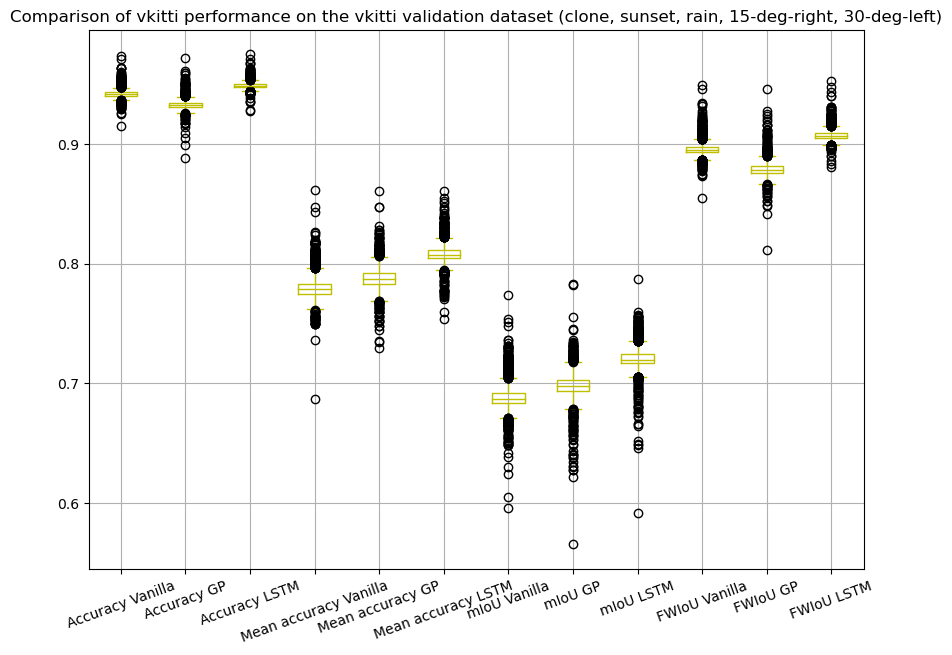
\includegraphics[width=12cm]{images/vkitti_validation_data_five_class_box_plot.png}
		\caption{Plotting of raw input image, ground truth and predicted output for vanilla, gp and lstm}
		\label{fig:performance_metric_unet}
	\end{figure}
	
	\begin{figure}
		\centering
		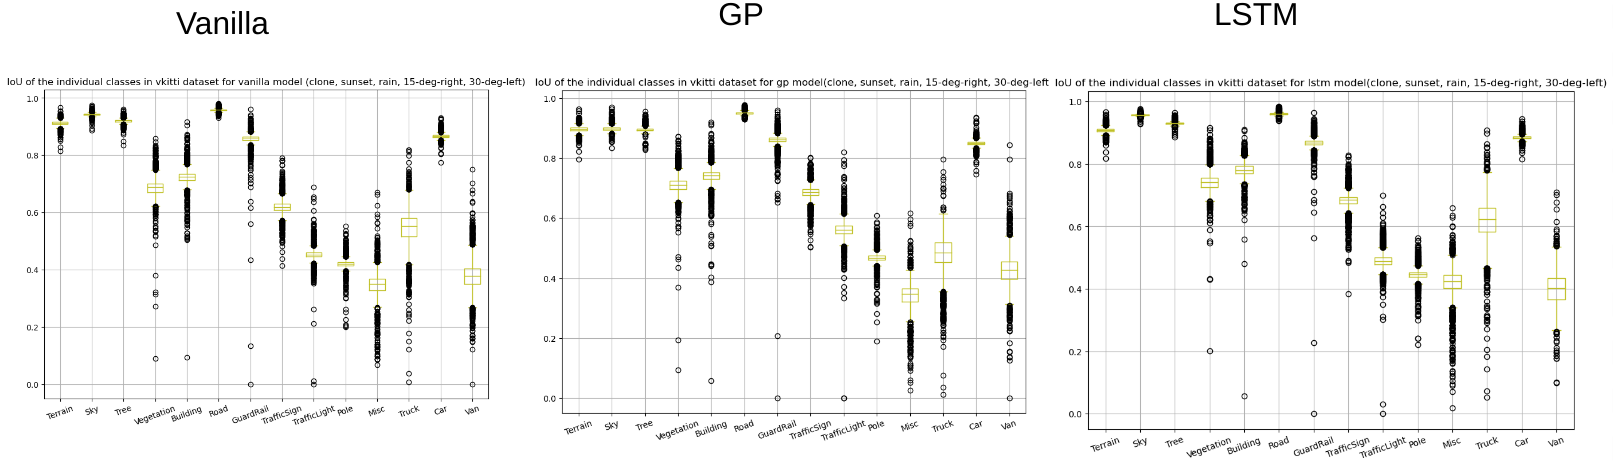
\includegraphics[width=19cm]{images/IoU_five.png}
		\caption{Plotting of raw input image, ground truth and predicted output for vanilla, gp and lstm}
		\label{fig:performance_metric_three_classes_unet_five}
	\end{figure}
	
%	\newpage
%	
%	\section{Benchmarking of results for scannet dataset and vkitti dataset}
%	
%	{ \bf Scannet dataset}
%	
%	The table \ref{table:scannet_benchmark} lists all the state of the art semantic segmentation model performance. The best average iou for the entire scannet dataset is 0.745. In this model 
%	
%	The pixel accuracy is 50.96\% for the validation dataset. The is due to the presence of large number of classes with unequal pixel distribution. However, the IoU for the Wall, Floor and Mattress is high at 0.56, 0.608, 0.382 due to the high pixel distribution for these classes. Frequency weighted IoU take into account the unequal pixel distribution and the values stand at 0.3531. The predicted and the ground truth pixel distribution is presented in the Fig \ref{fig:y_gt_pred_vanilla}.
%	
%	The pixel accuracy is 50.96\% for the validation dataset. The is due to the presence of large number of classes with unequal pixel distribution. However, the IoU for the Wall, Floor and Mattress is high at 0.56, 0.608, 0.382 due to the high pixel distribution for these classes. Frequency weighted IoU take into account the unequal pixel distribution and the values stand at 0.3531. The predicted and the ground truth pixel distribution is presented in the Fig \ref{fig:y_gt_pred_vanilla}. Frequency weighted IoU take into account the unequal pixel distribution and the values stand at 0.3531. The predicted and the ground truth pixel distribution is presented in the Fig \ref{fig:y_gt_pred_vanilla}.
%	Frequency weighted IoU take into account the unequal pixel distribution and the values stand at 0.3531. The predicted and the ground truth pixel distribution is presented in the Fig \ref{fig:y_gt_pred_vanilla}.Frequency weighted IoU take into account the unequal pixel distribution and the values stand at 0.3531. The predicted and the ground truth pixel distribution is presented in the Fig \ref{fig:y_gt_pred_vanilla}.
	
%	\begin{table}[h]
%		\begin{center}
%			\begin{tabular}{ | l | l | l | l| p{4cm} |}
%				\hline
%				
%				\cellcolor{purple!30}Method & \cellcolor{purple!30}Avg iou & \cellcolor{purple!30} Pixel Accuracy & \cellcolor{purple!30} Mean Pixel Accuracy & \cellcolor{purple!30} FwIoU \\ \hline
%				
%				Virtual MVFusion (R) & 0.745 & - & - & -  \\ \hline
%				BPNet\_2D & 0.67 & - & - & -  \\ \hline
%				CU-Hybrid-2D Net & 0.636  & - & - & -  \\ \hline
%				CMX & 0.613 & - & - & -  \\ \hline
%				DMMF\_3d & 0.605 & - & -  & - \\ \hline
%				MCA-Net & 0.595 & - & -  & - \\ \hline
%				RFBNet & 0.592 & - & -  & - \\ \hline
%				DCRedNet & 0.583 & -  & - & - \\ \hline
%				SSMA & 0.577 & - & -  & - \\ \hline
%				SN\_RN152pyrx8\_RVC & 0.546 & - & - & - \\ \hline
%				FuseNet & 0.535 & - & -  & - \\ \hline
%				AdapNet++ & 0.503 & - & -  & - \\ \hline
%				3DMV (2d proj) & 0.498 & - & - & - \\ \hline
%				MSeg1080\_RVC & 0.485 & -  & - & - \\ \hline
%				ILC-PSPNet & 0.475 & - & - & - \\ \hline
%				Enet & 0.376 & - & - & - \\ \hline
%				ScanNet & 0.33 & - & - & - \\ \hline
%				LSTM Unet & 0.145 & - & -  & - \\ \hline
%				GP Unet & 0.1161  & - & - & - \\ \hline
%				Vanilla Unet & 0.112 & - & - & - \\ \hline
%			
%				\hline
%			\end{tabular}
%			\caption{Comparison of model performance on the Scannet data}
%			\label{table:scannet_benchmark}
%		\end{center}
%	\end{table}	
%	
%	\newpage
%	
%	{ \bf Vkitti dataset, refer: https://arxiv.org/pdf/2006.04080v2.pdf}
%	
%	The pixel accuracy is 50.96\% for the validation dataset. The is due to the presence of large number of classes with unequal pixel distribution. However, the IoU for the Wall, Floor and Mattress is high at 0.56, 0.608, 0.382 due to the high pixel distribution for these classes. Frequency weighted IoU take into account the unequal pixel distribution and the values stand at 0.3531. The predicted and the ground truth pixel distribution is presented in the Fig \ref{fig:y_gt_pred_vanilla}. Frequency weighted IoU take into account the unequal pixel distribution and the values stand at 0.3531. The predicted and the ground truth pixel distribution is presented in the Fig \ref{fig:y_gt_pred_vanilla}.
%	Frequency weighted IoU take into account the unequal pixel distribution and the values stand at 0.3531. The predicted and the ground truth pixel distribution is presented in the Fig \ref{fig:y_gt_pred_vanilla}.Frequency weighted IoU take into account the unequal pixel distribution and the values stand at 0.3531. The predicted and the ground truth pixel distribution is presented in the Fig \ref{fig:y_gt_pred_vanilla}.
	
%	\begin{table}[h]
%		\begin{center}
%			\begin{tabular}{ | l | l | l | l| p{4cm} |}
%				\hline
%				
%				\cellcolor{purple!30}Method & \cellcolor{purple!30}Avg iou & \cellcolor{purple!30} Pixel Accuracy & \cellcolor{purple!30} Mean Pixel Accuracy & \cellcolor{purple!30} FwIoU \\ \hline
%				
%				Virtual MVFusion (R) & 0.745 & - & - & -  \\ \hline
%				BPNet\_2D & 0.67 & - & - & -  \\ \hline
%				CU-Hybrid-2D Net & 0.636  & - & - & -  \\ \hline
%				CMX & 0.613 & - & - & -  \\ \hline
%				DMMF\_3d & 0.605 & - & -  & - \\ \hline
%				MCA-Net & 0.595 & - & -  & - \\ \hline
%				RFBNet & 0.592 & - & -  & - \\ \hline
%				DCRedNet & 0.583 & -  & - & - \\ \hline
%				SSMA & 0.577 & - & -  & - \\ \hline
%				SN\_RN152pyrx8\_RVC & 0.546 & - & - & - \\ \hline
%				FuseNet & 0.535 & - & -  & - \\ \hline
%				AdapNet++ & 0.503 & - & -  & - \\ \hline
%				3DMV (2d proj) & 0.498 & - & - & - \\ \hline
%				MSeg1080\_RVC & 0.485 & -  & - & - \\ \hline
%				ILC-PSPNet & 0.475 & - & - & - \\ \hline
%				Enet & 0.376 & - & - & - \\ \hline
%				ScanNet & 0.33 & - & - & - \\ \hline
%				Vanilla Unet & 0.112 & - & - & - \\ \hline
%				GP Unet & 0.1161  & - & - & - \\ \hline
%				LSTM Unet & 0.145 & - & -  & - \\ \hline
%				\hline
%			\end{tabular}
%			\caption{Comparison of model performance on the Scannet data}
%			\label{table:LSTM_conti_seq}
%		\end{center}
%	\end{table}
    
\end{document}
